\chapter{Design} \label{chap:design}

%\version{v1.10.2015}

\section*{}
\section{System Architecture \cite{arch}}

\begin{figure}[H]
	\begin{center}
		{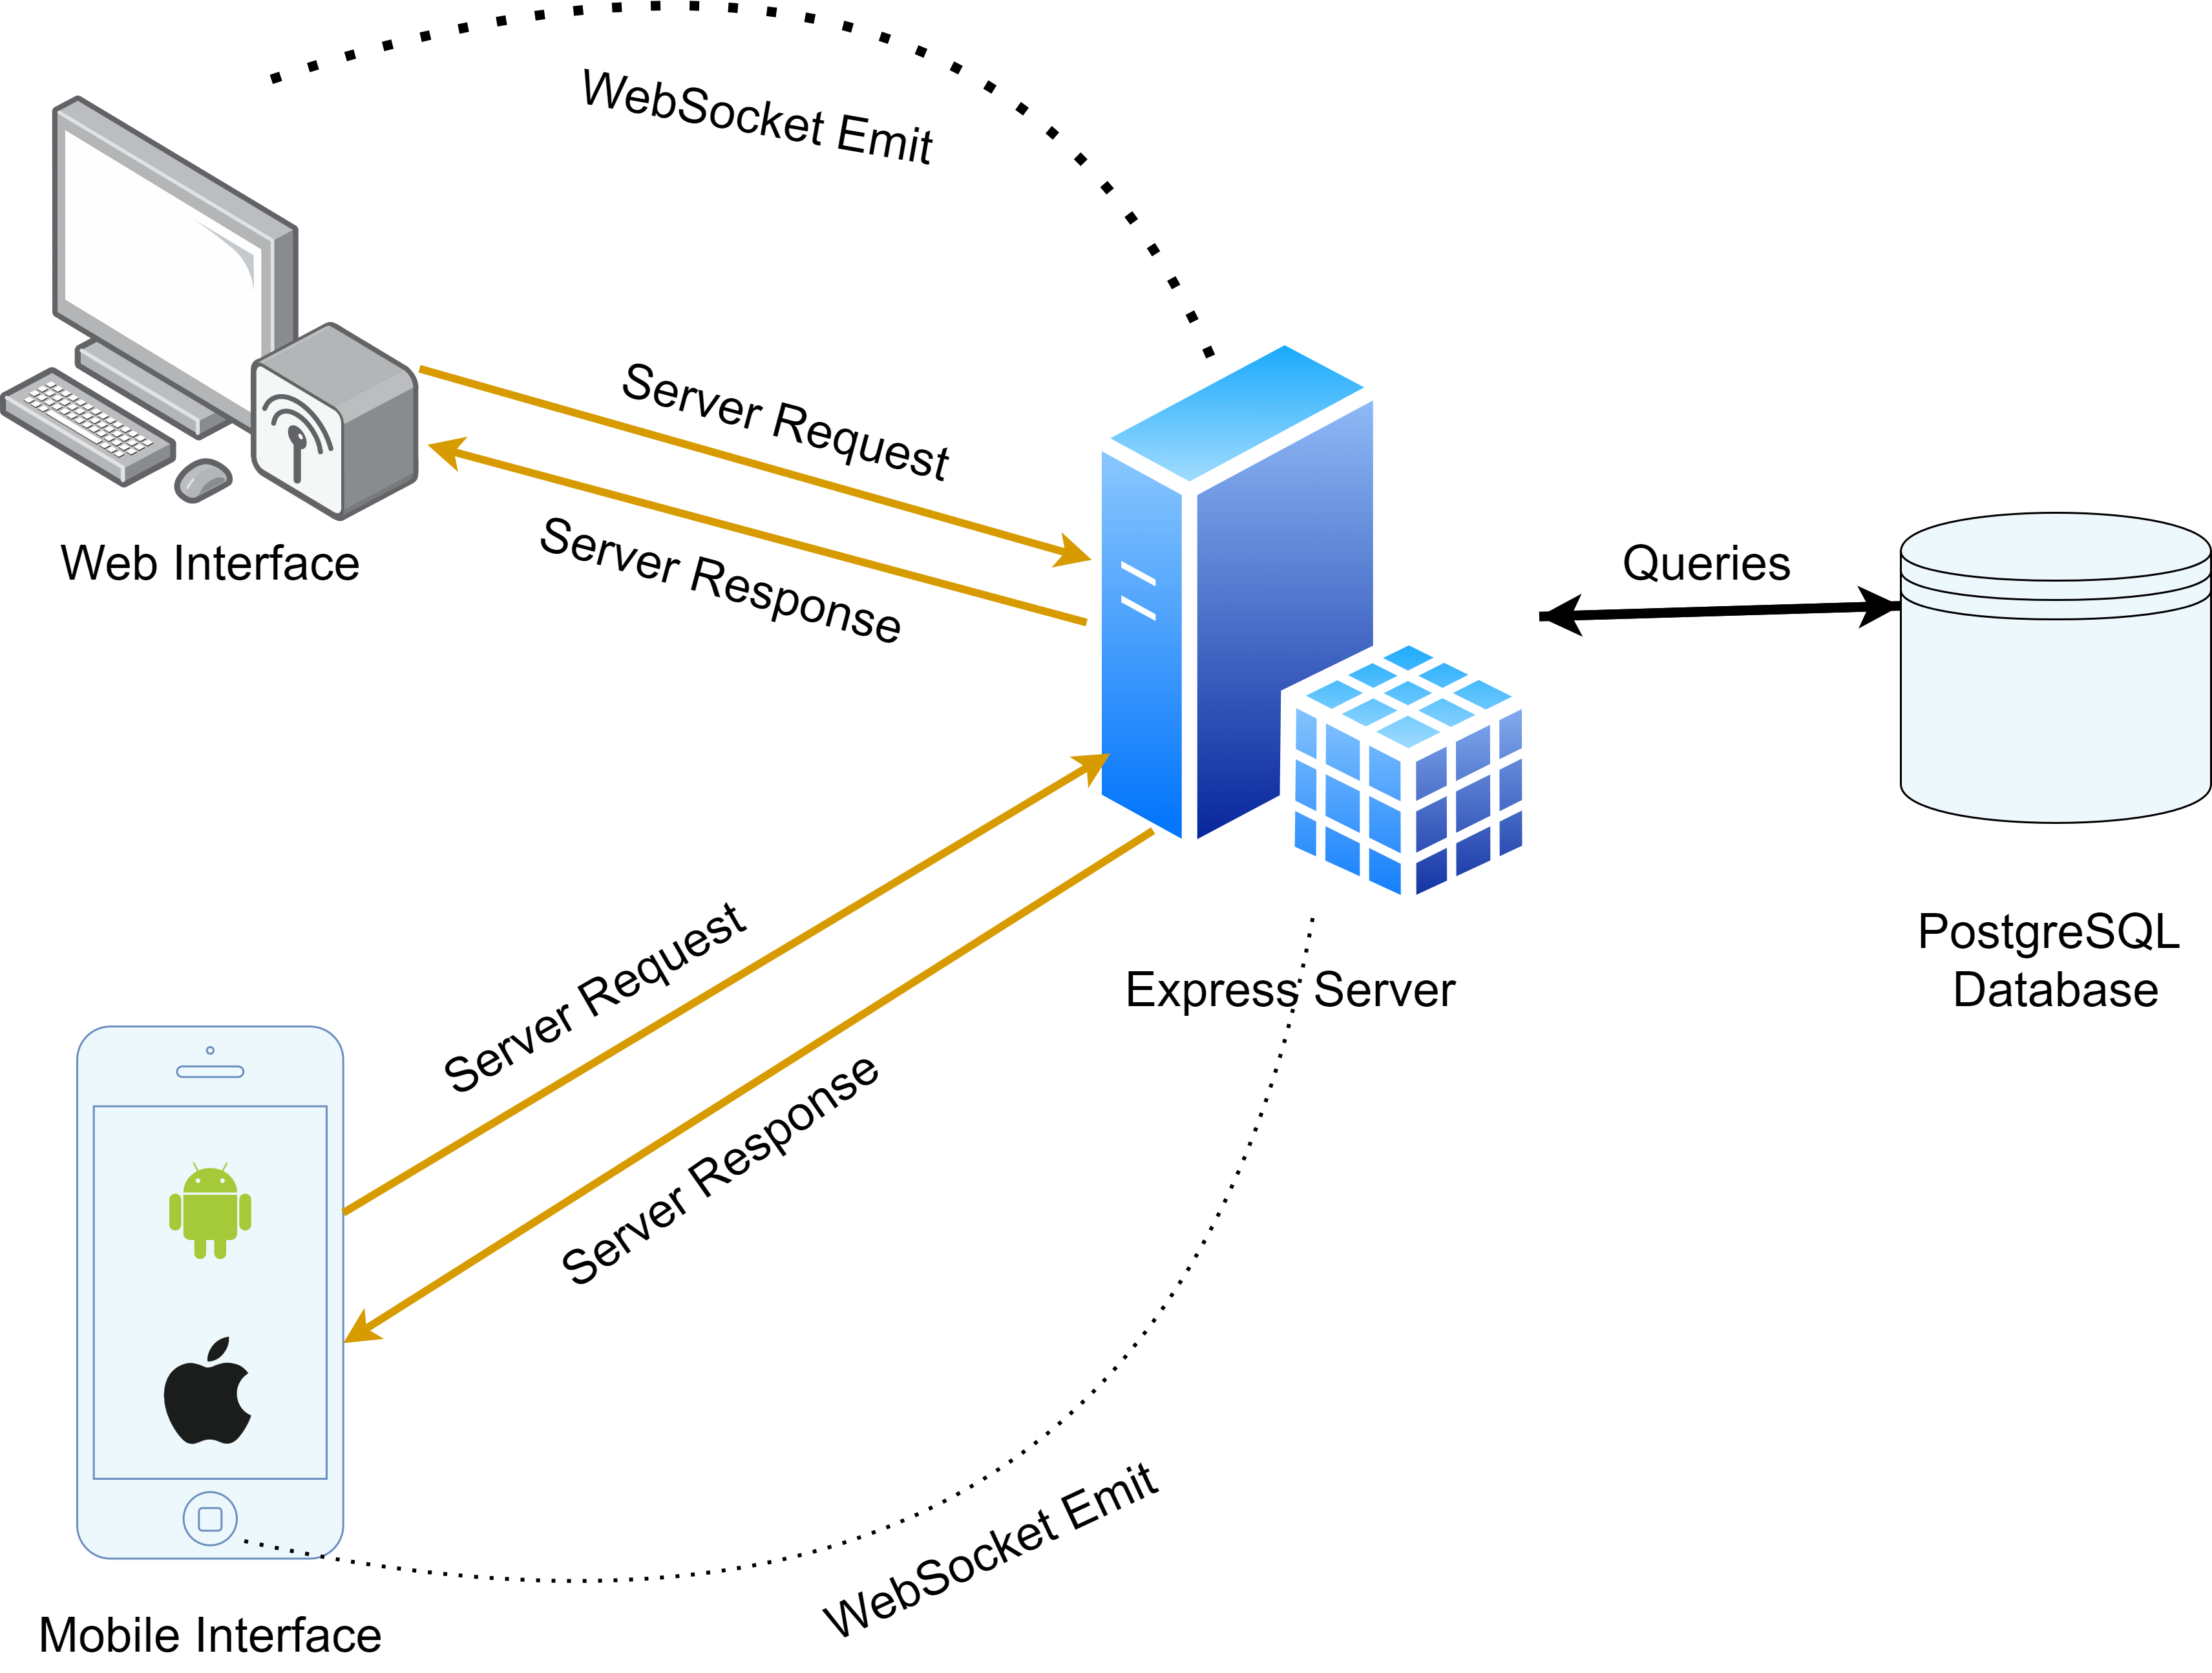
\includegraphics[scale=0.4]{figures/architecture.png}}
		\caption{Architecture Diagram}
	\end{center}
\end{figure}

\section{Design Constraints}
The database is hosted at Heroku Server \cite{heroku}. This server limits the connections up to 20 and maximum of 10,000 rows. For a real-world implementation, this can cause issue as the space would run out quickly and maximum of 20 users will be able to use the application. However, since this approach has no expenses, it saves the project from monetary investments. The middle server is also hosted on a free solution on Heroku which also runs at a slower speed rather than a paid one.

\section{Design Methodology}

Functional Decomposition \cite{decom} is followed for the creation of the design as the front-end was designed first which holds all the functionality. After the front-end was successfully designed, only than the database was designed. To design the front-end for mobile, other relative applications such as real-estate, e-commerce apps were looked at. The screens and components that were being repeated over there were made compulsory for this application to have. Since on the server, mobile and web application, screens and components were designed using functional components, it is safe to say it followed the structured methodology. However, for database, a lot of fields and entities are involved which fall under the object-oriented methodology.

\section{High Level Design}
We have shown the system architecture design in Section 4.1. Now we are going to elaborate the working with the help of package diagram and deployment diagram. We have tried to present our system in the most understandable manner.

\subsection{Conceptual or Logical View}

Authentication Package needs Login, Forget and Reset Package for successful login. Authentication is same for Customer, Admin, Owner and Customer Sales Agent. This package will be further elaborated in next section with the help of interaction diagram.
\begin{figure}[H]
	\begin{center}
		{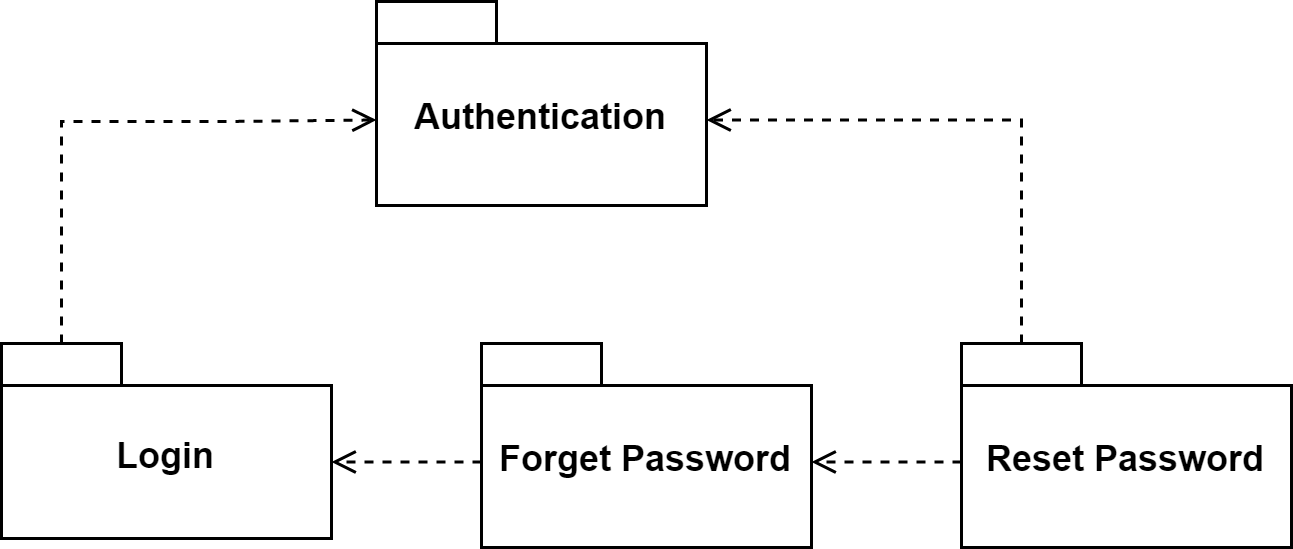
\includegraphics[scale=0.8]{figures/web Concept/web-auth package.png}}
		\caption{Authentication Package}
	\end{center}
\end{figure}

In Customer Relation Management Portal we have Disputes Package that presents list of assigned disputes by using Chat package to chat with the customer and Profile package to edit profile.
\begin{figure}[H]
	\begin{center}
		{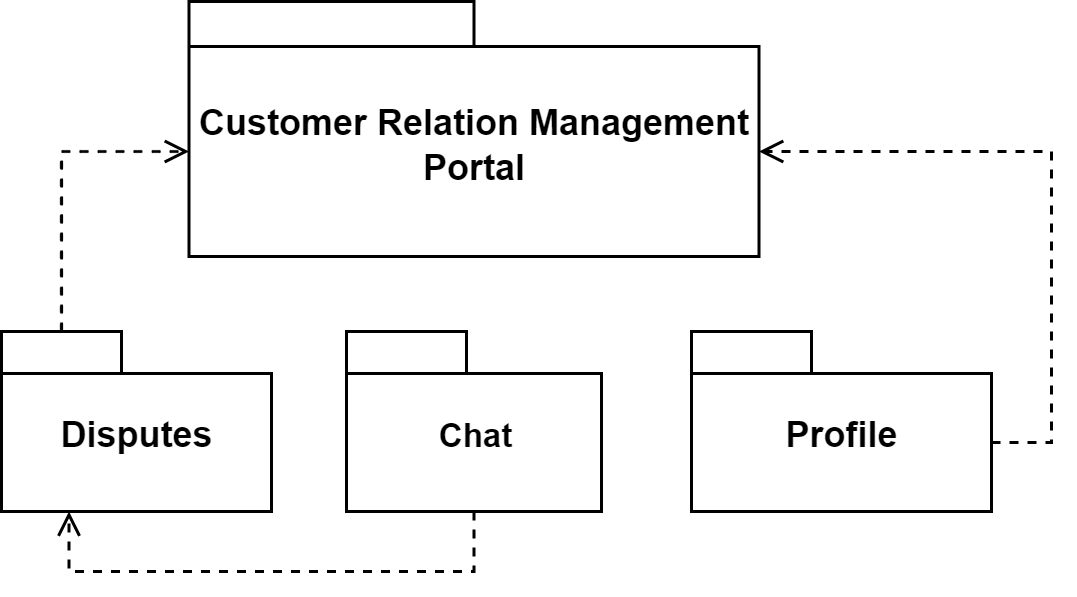
\includegraphics[scale=0.8]{figures/web Concept/web-crm_package.png}}
		\caption{CRM Portal Package}
	\end{center}
\end{figure}

Admin portal Package includes Projects, Transaction, Meeting etc, for full functionality.
\begin{figure}[H]
	\begin{center}

		{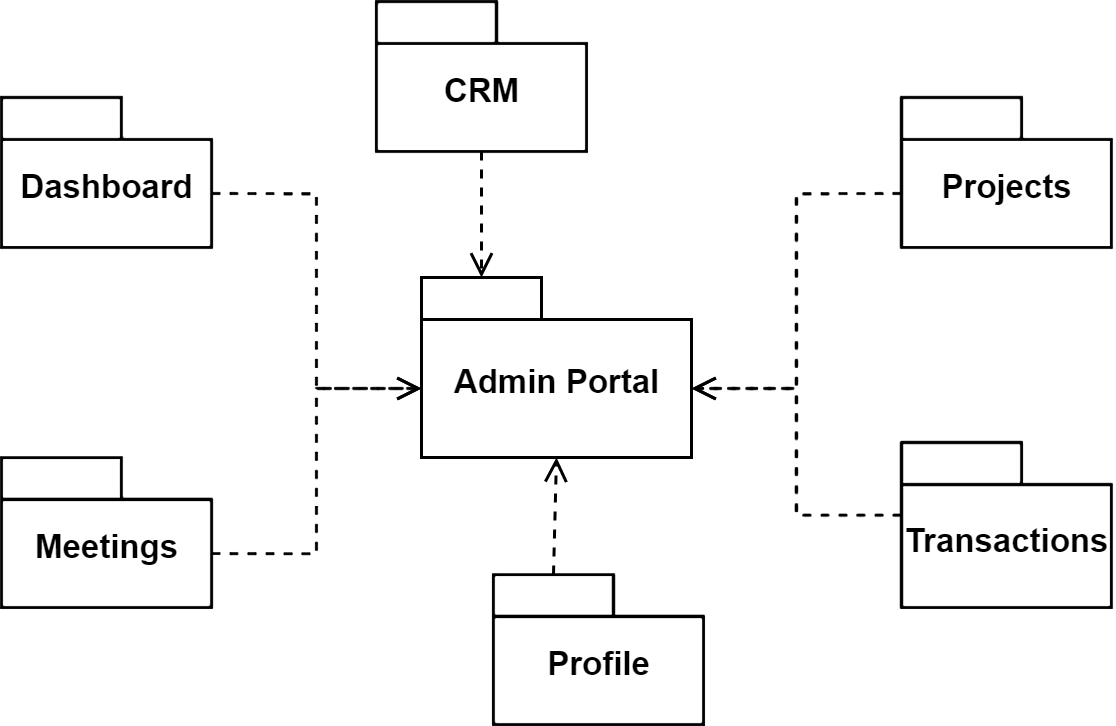
\includegraphics[scale=1]{figures/web Concept/web-admin_package.png}}
		\caption{Admin Portal Package}
	\end{center}
\end{figure}

By using below packages we get complete web portal package that redirects users to their specific Portal according to their roles.
\begin{figure}[H]
	\begin{center}
		{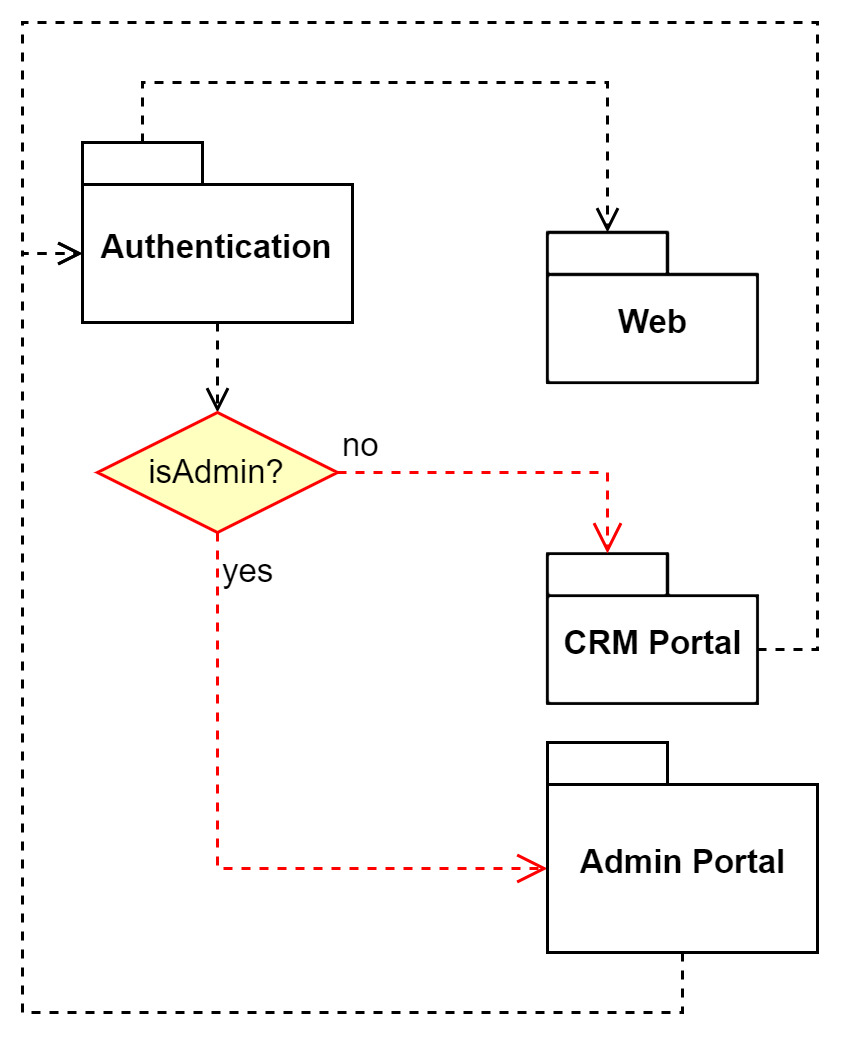
\includegraphics[scale=1.2]{figures/web Concept/web-web portal.png}}
		\caption{Complete Web Package}
		\label{web_package}
	\end{center}
\end{figure}


\newpage
\subsection{Process}
\begin{figure}[H]
	\begin{center}
		{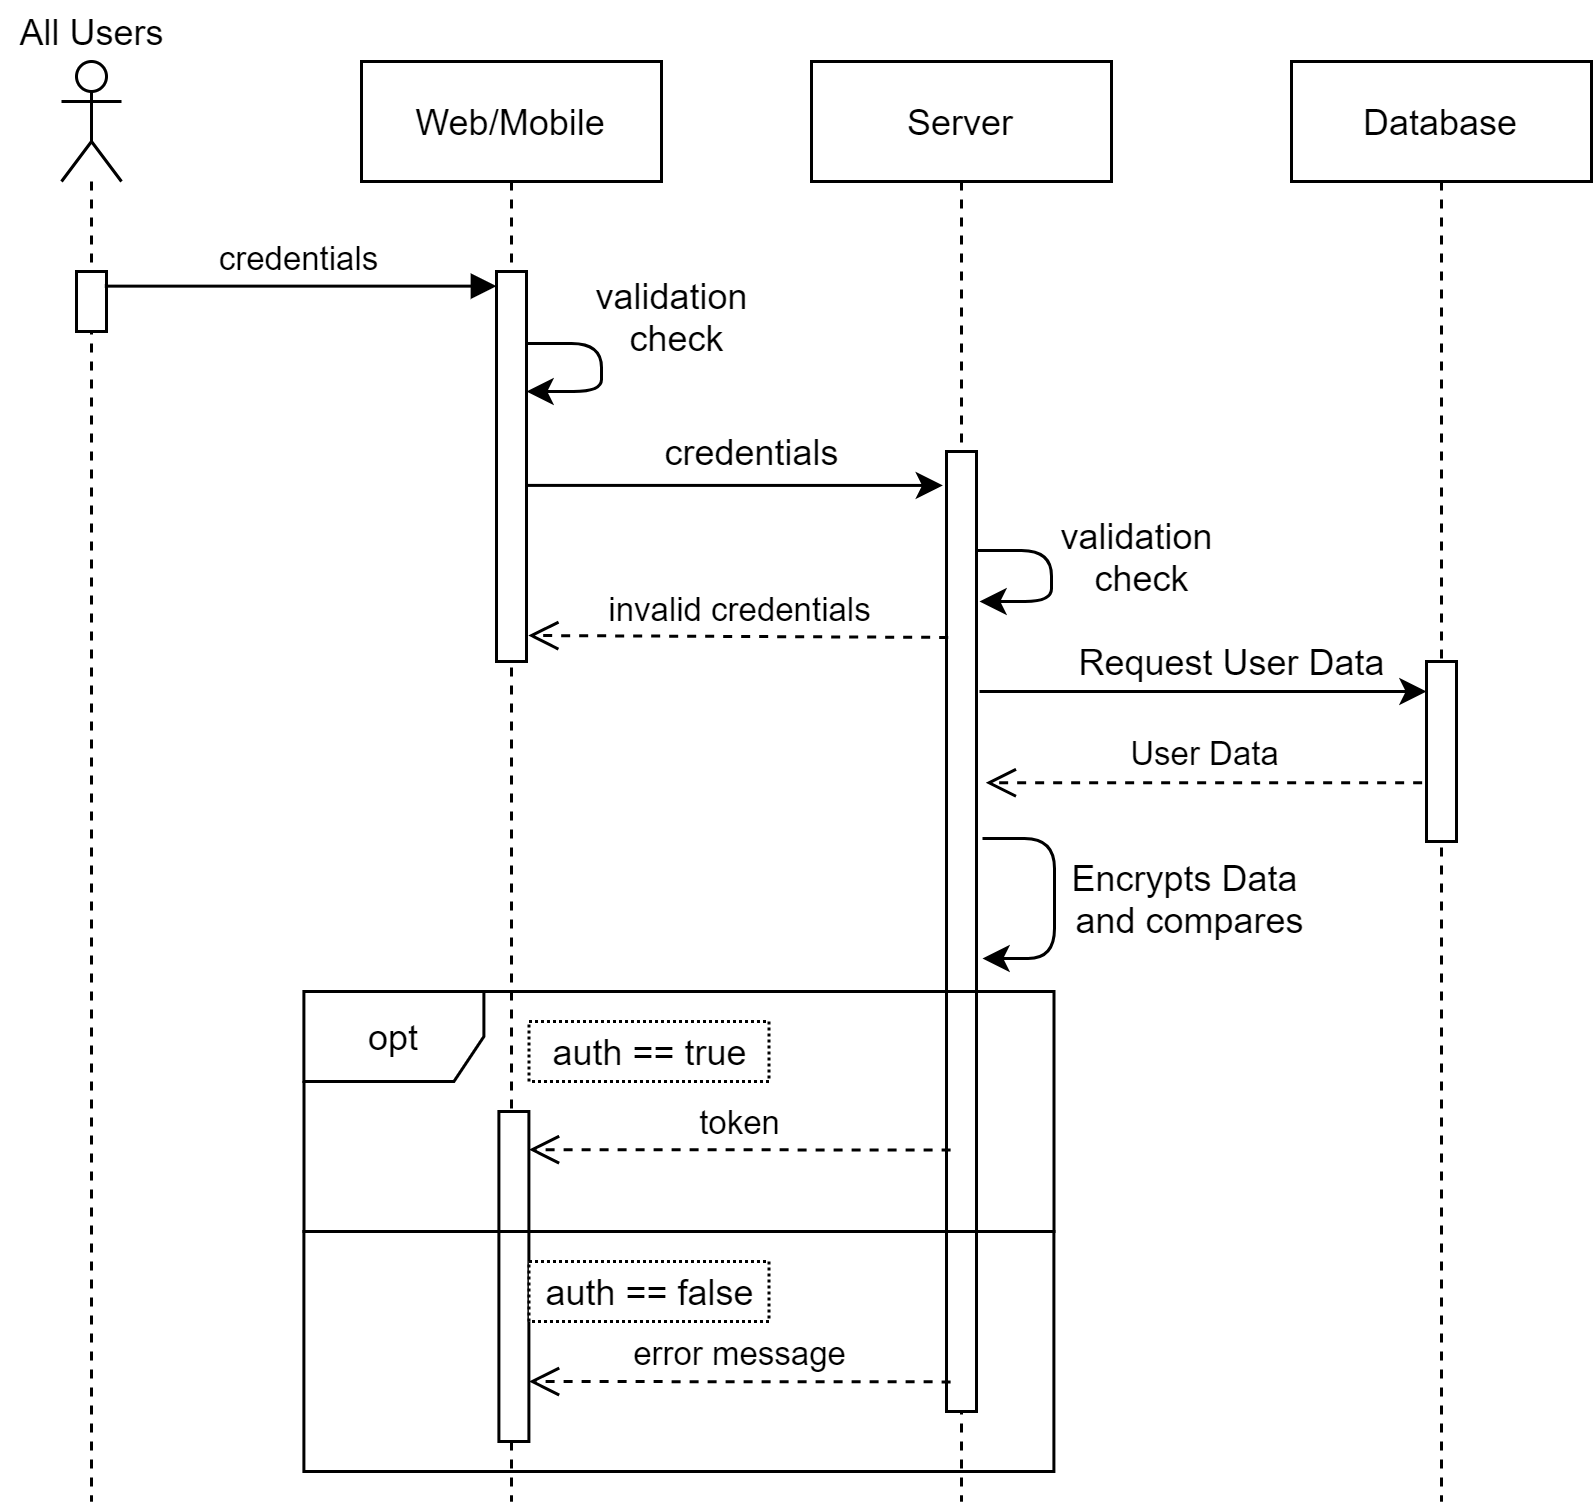
\includegraphics[scale=1.2]{Sequence Diagrams/Auth_1.png}}
		\caption{Login}
	\end{center}
\end{figure}

\newpage
\begin{figure}[H]
	\begin{center}
		{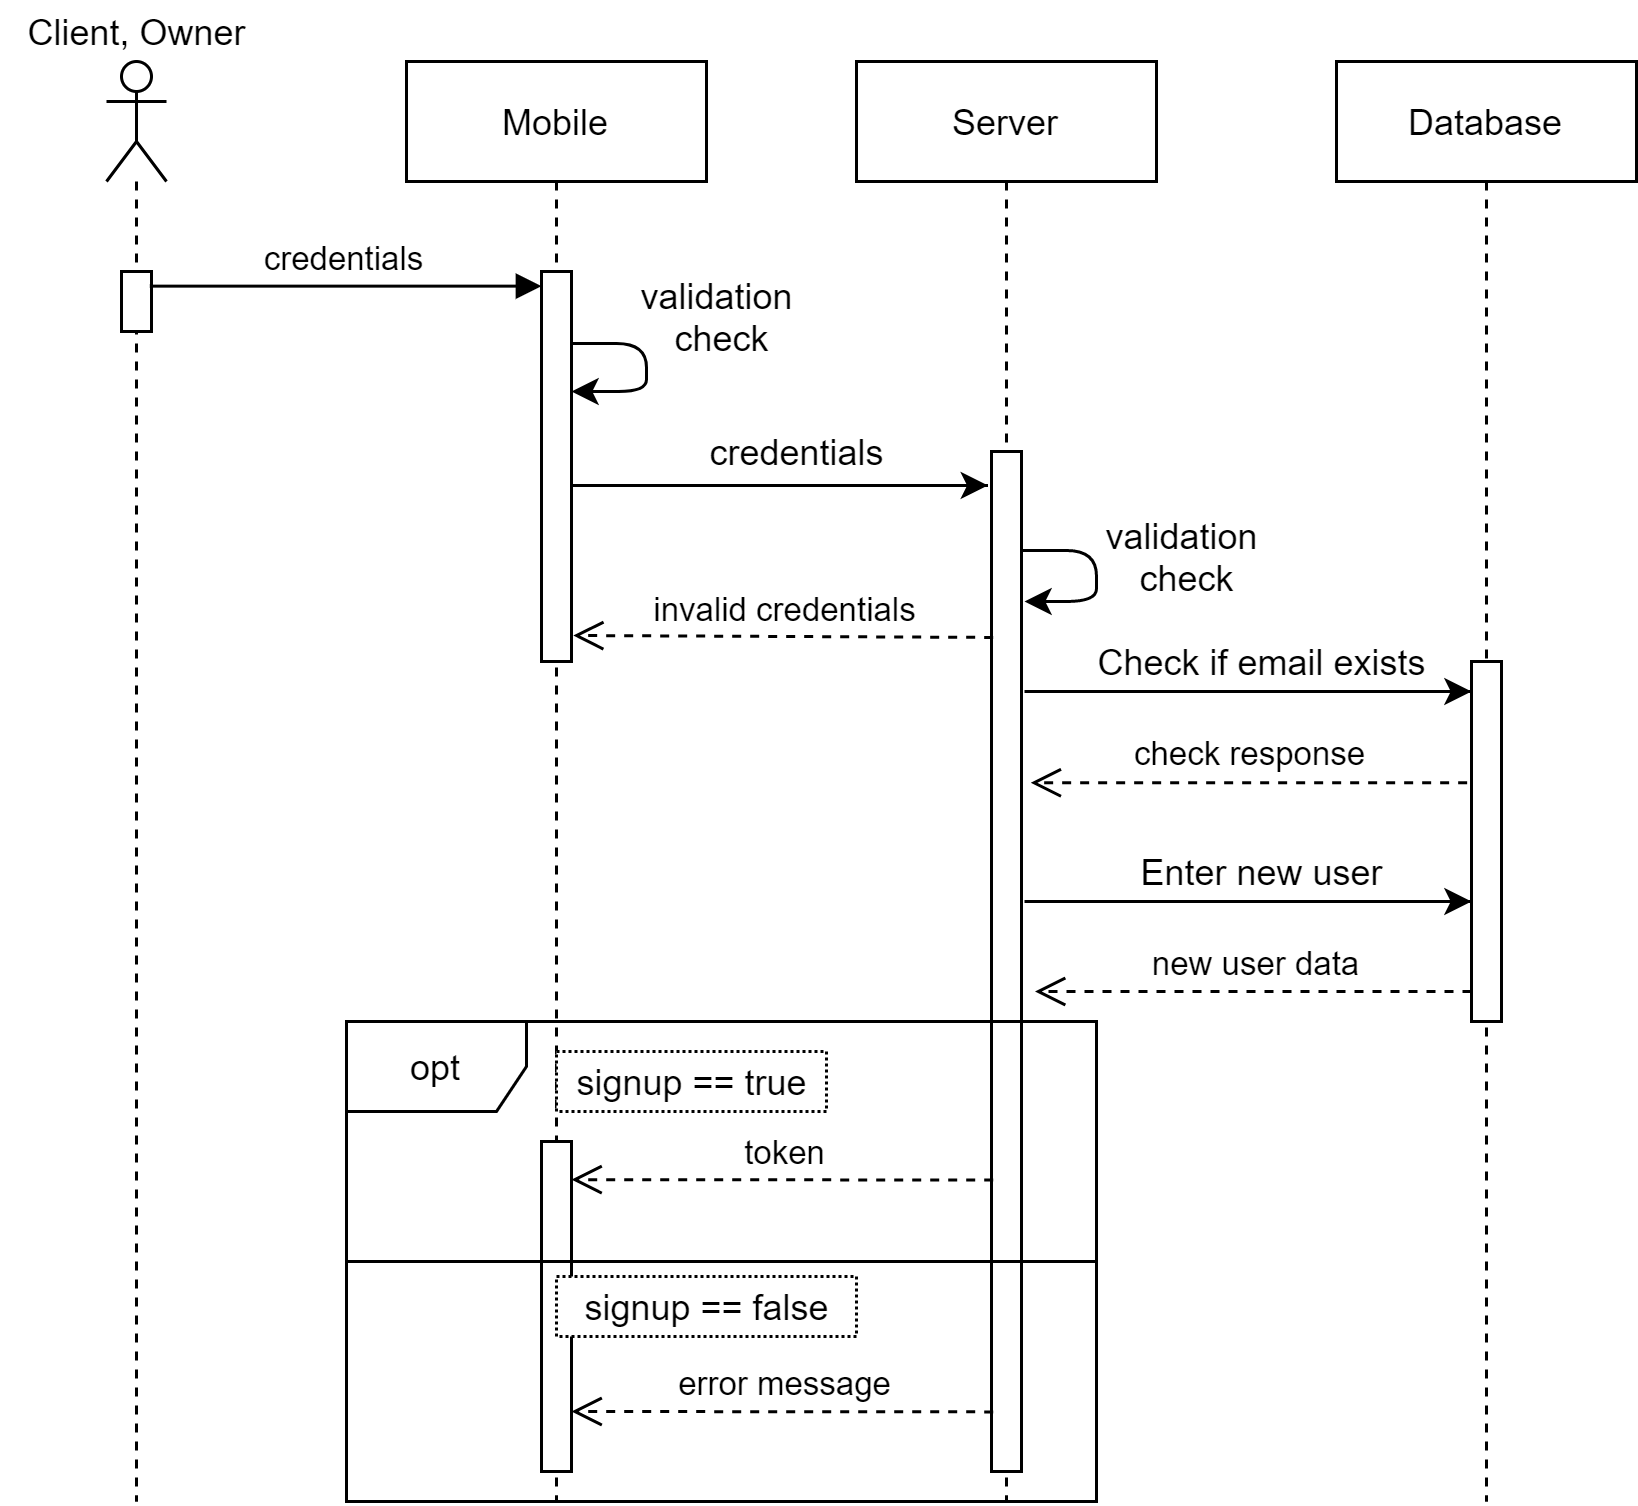
\includegraphics[scale=1.2]{Sequence Diagrams/Auth_2.png}}
		\caption{Register}
	\end{center}
\end{figure}

\newpage
\begin{figure}[H]
	\begin{center}
		{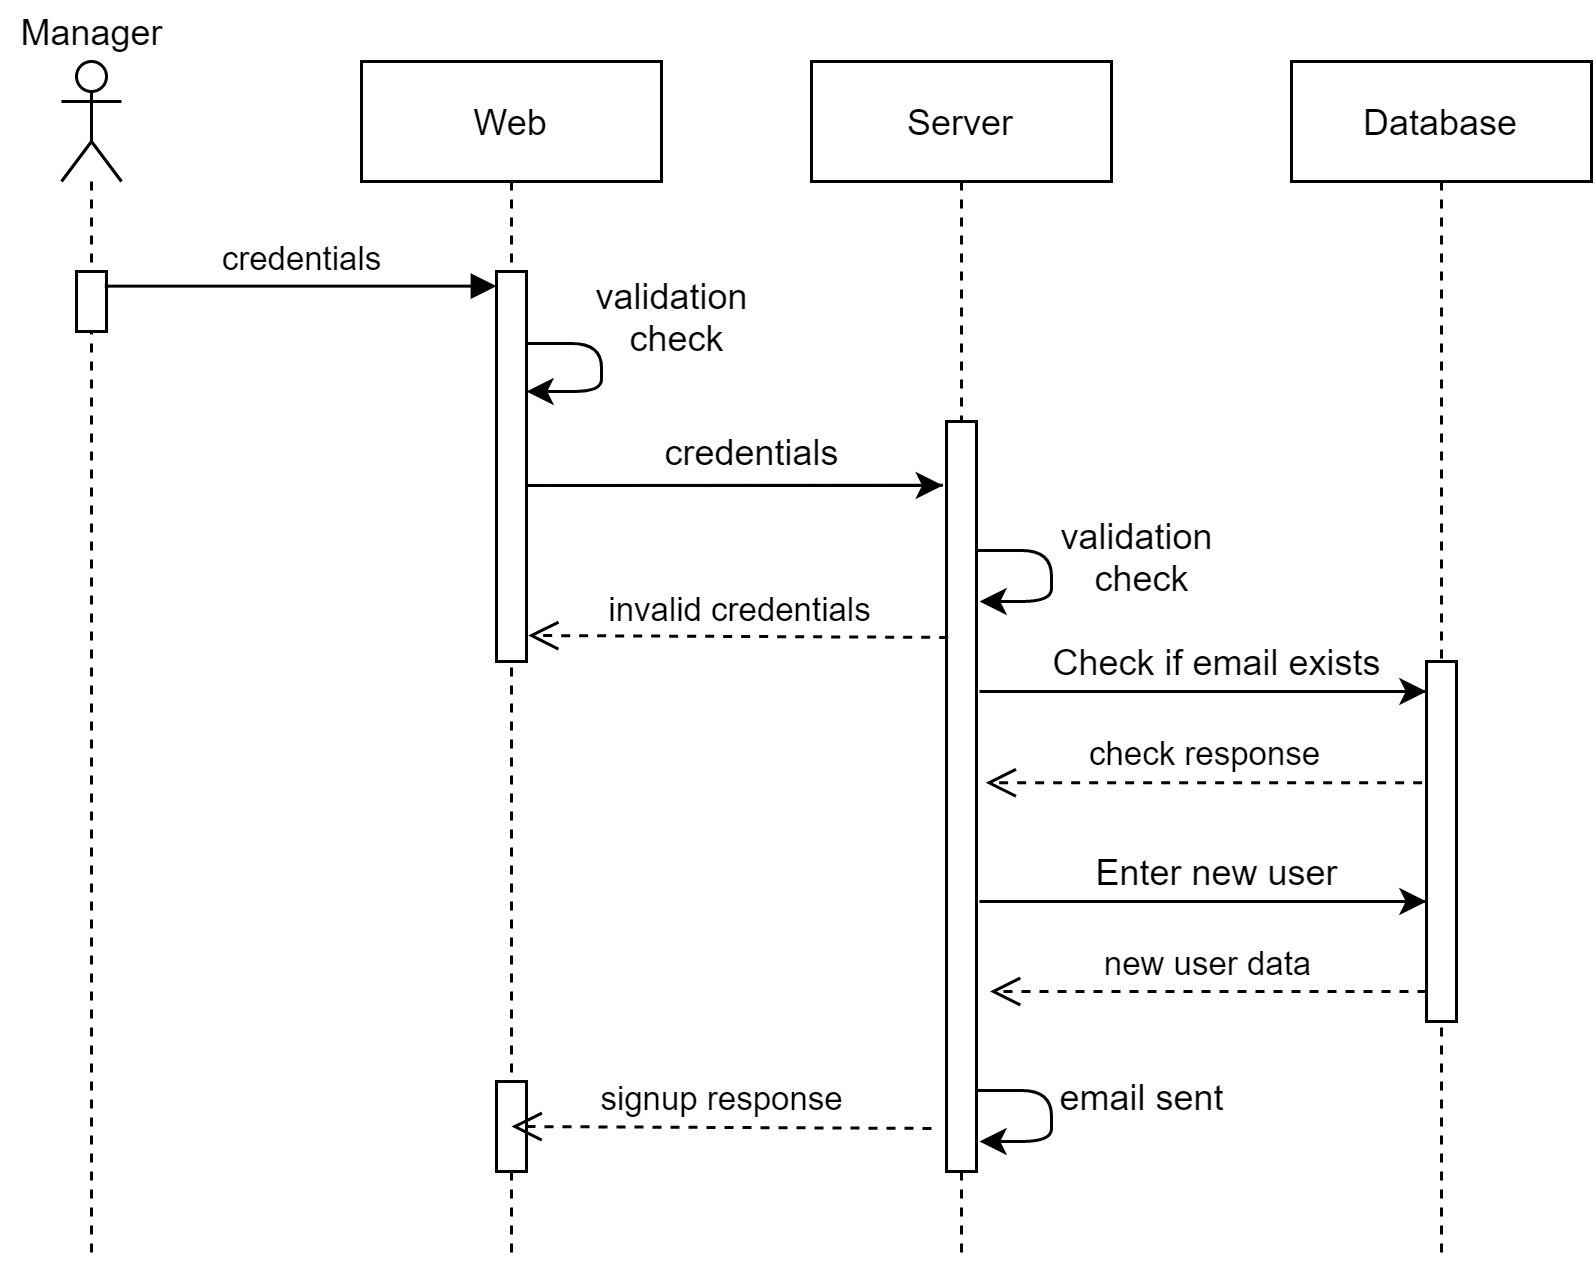
\includegraphics[scale=1.2]{Sequence Diagrams/New CRO.png}}
		\caption{New CRO}
	\end{center}
\end{figure}

\newpage
\begin{figure}[H]
	\begin{center}
		{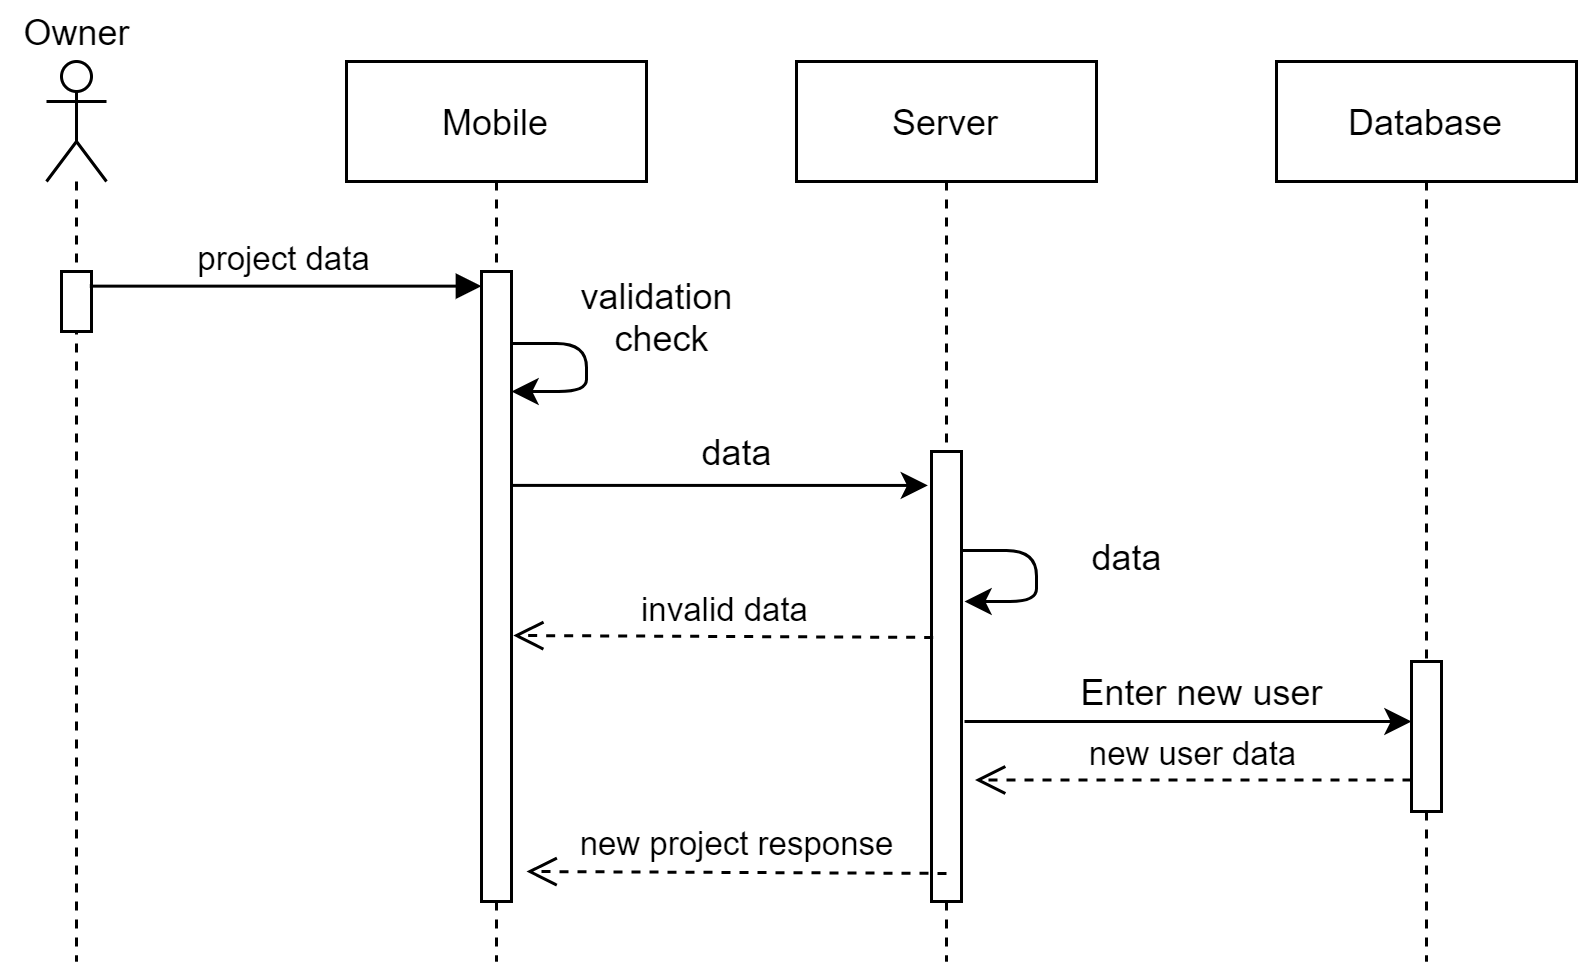
\includegraphics[scale=1.2]{Sequence Diagrams/New Project.png}}
		\caption{New Project}
	\end{center}
\end{figure}

\begin{figure}[H]
	\begin{center}
		{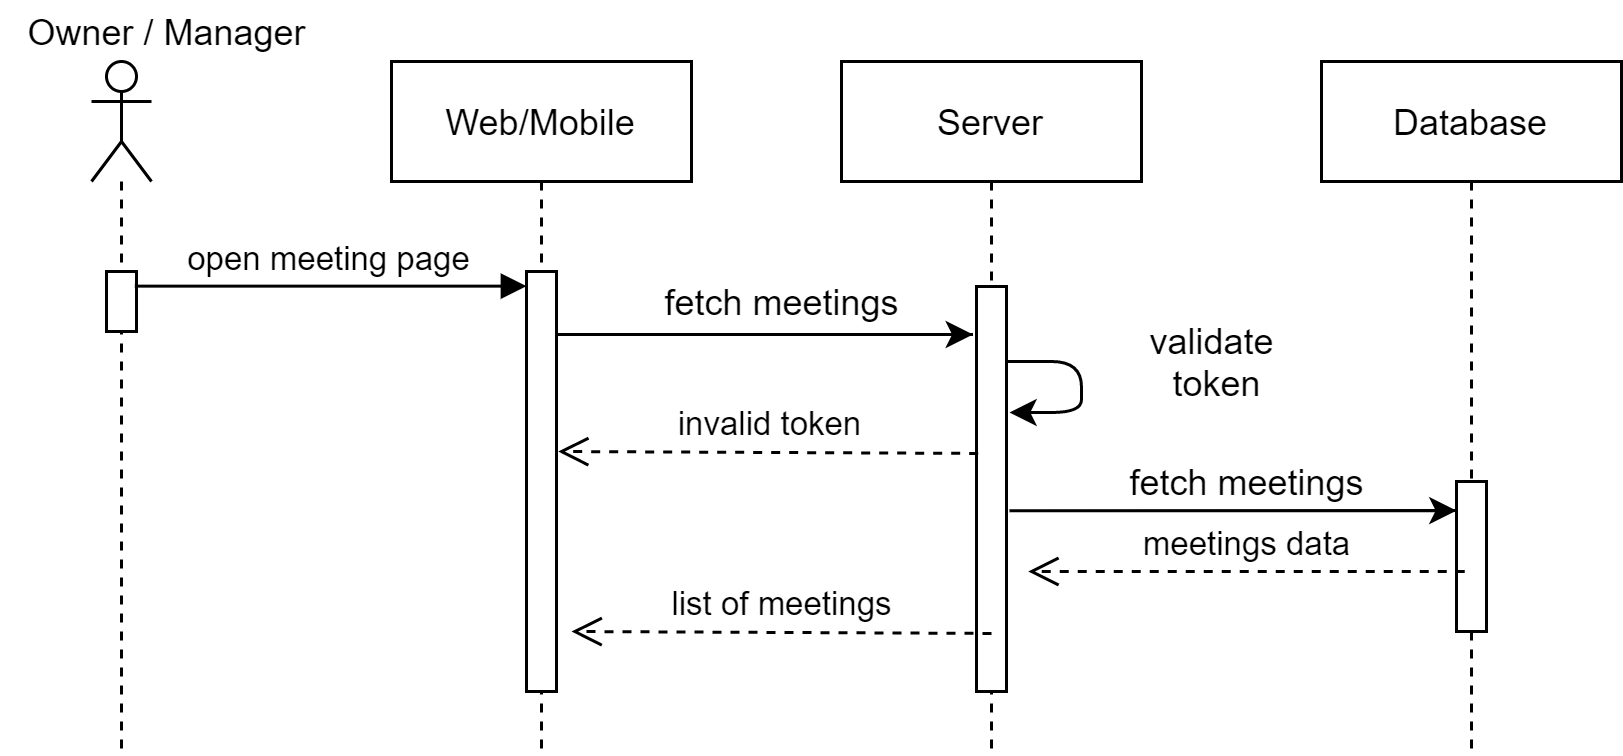
\includegraphics[scale=1.2]{Sequence Diagrams/Fetch Meetings.png}}
		\caption{Fetch Meetings}
	\end{center}
\end{figure}

\newpage
\begin{figure}[H]
	\begin{center}
		{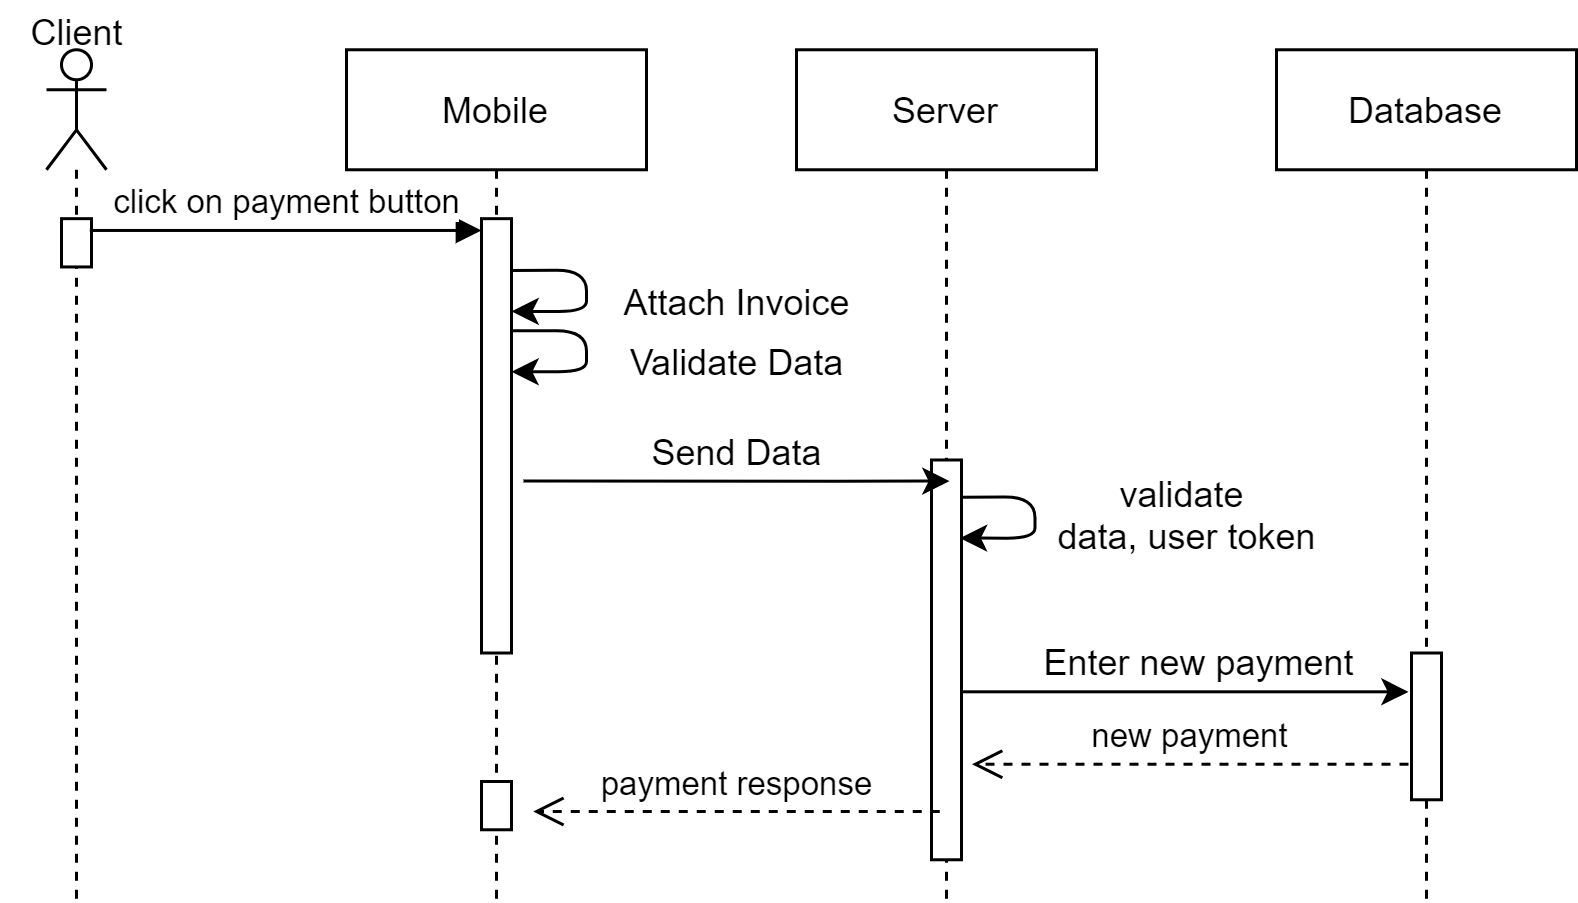
\includegraphics[scale=1.2]{Sequence Diagrams/Make Payment.png}}
		\caption{Make Payment}
	\end{center}
\end{figure}

\begin{figure}[H]
	\begin{center}
		{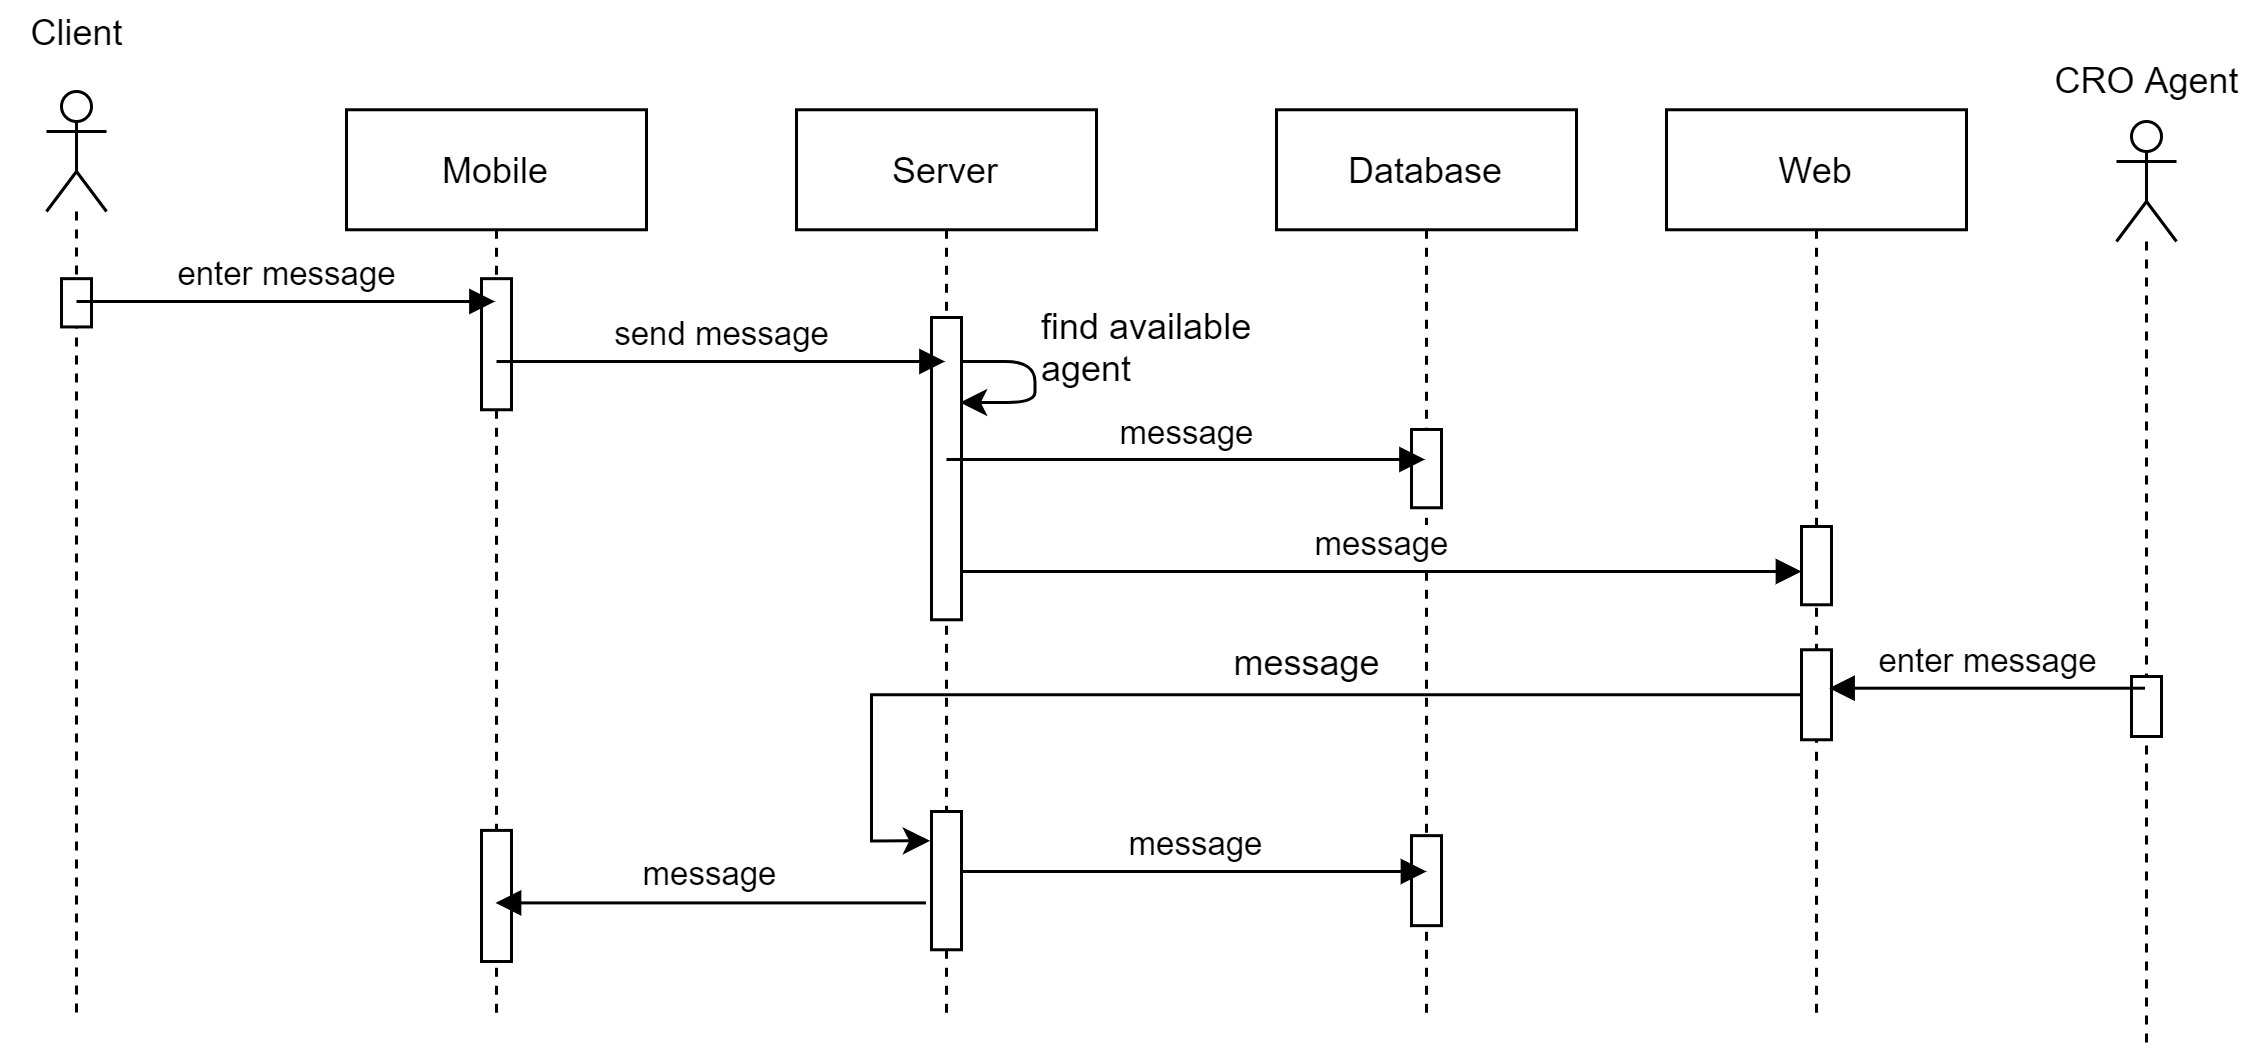
\includegraphics[scale=0.9]{Sequence Diagrams/Chat.png}}
		\caption{Chat}
	\end{center}
\end{figure}

\newpage
\begin{figure}[H]
	\begin{center}
		{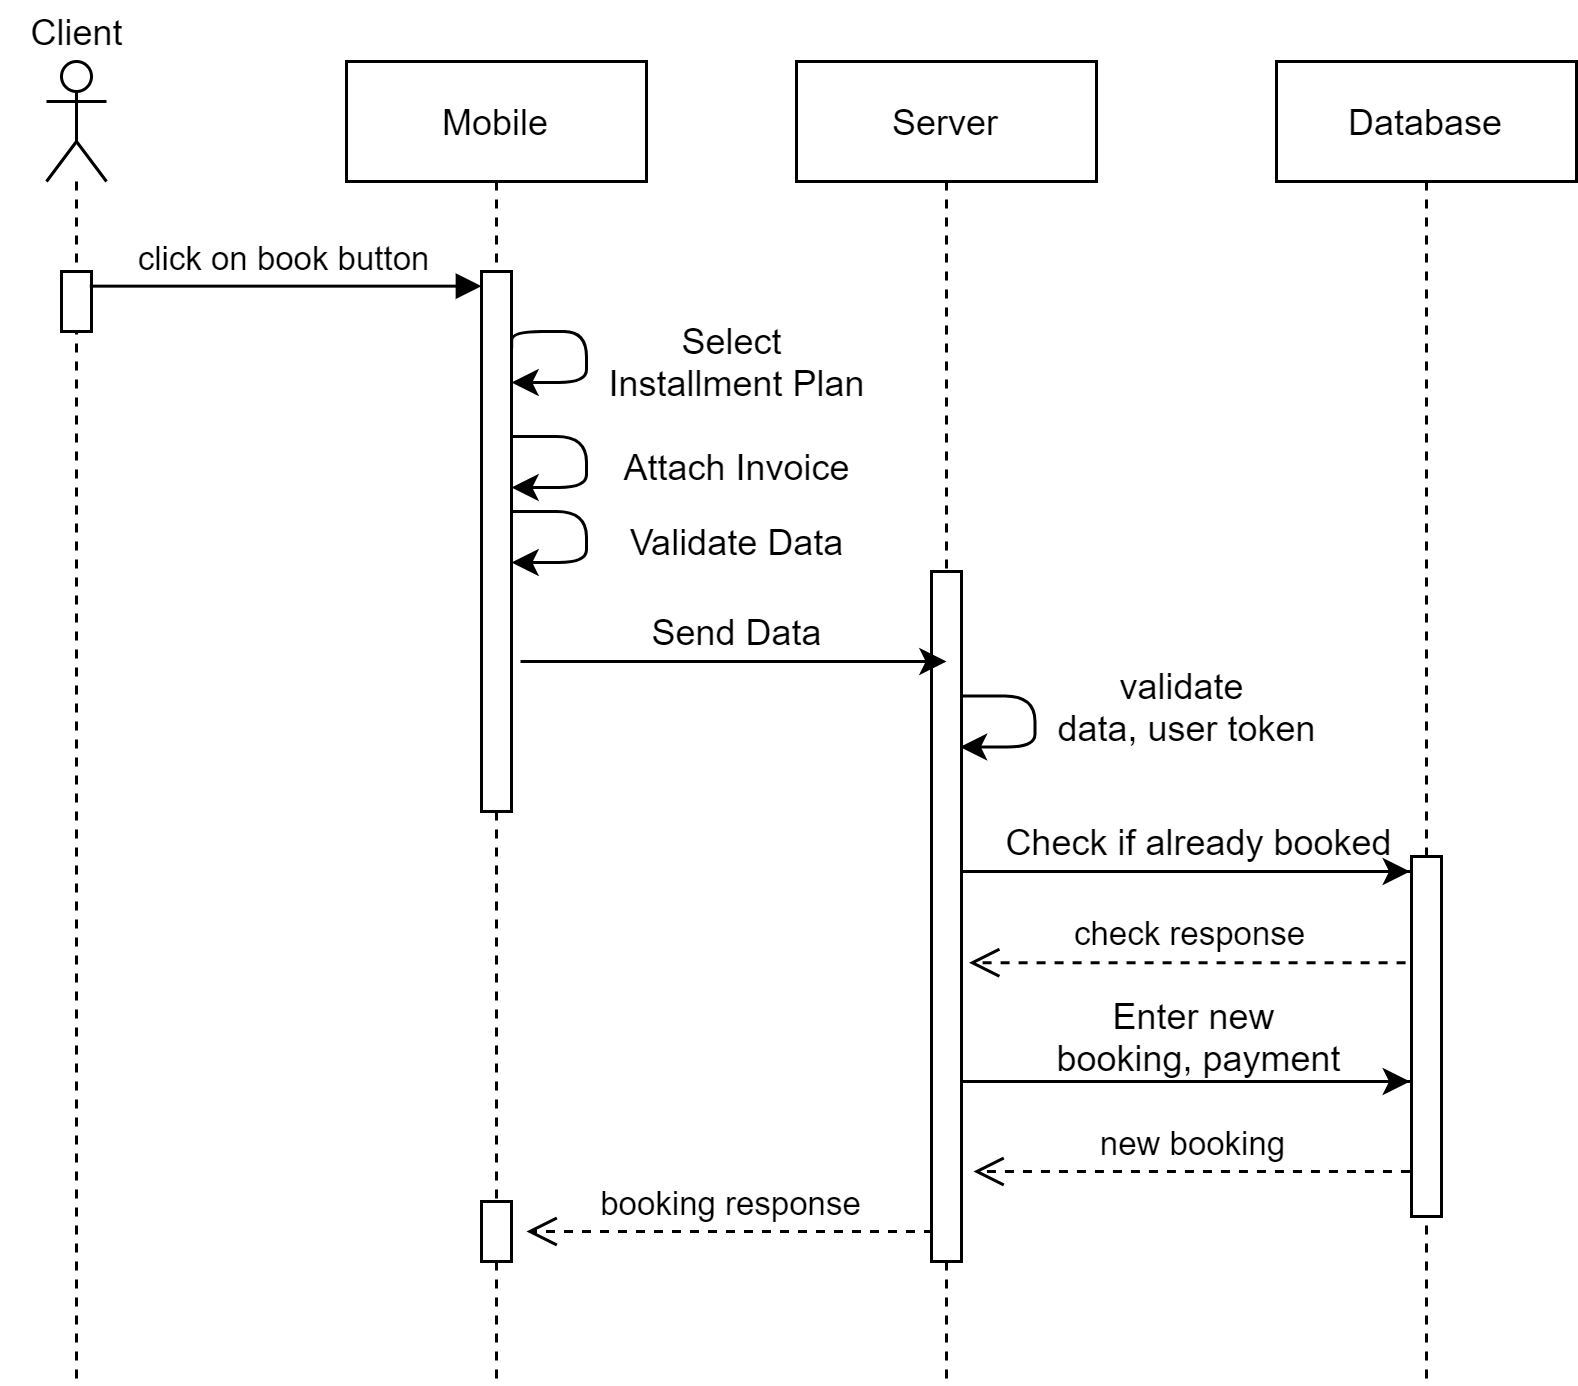
\includegraphics[scale=1.2]{Sequence Diagrams/Book Project.png}}
		\caption{Book Project}
	\end{center}
\end{figure}


\newpage
\subsection{Module}
We are following the standard model of react directory structure.The visual representation is shown below.
\hypertarget{mylink}{}
\begin{verbatim}
api/
	APIUtils.js
	APIUtils.test.js
	ProfileAPI.js
	UserAPI.js
components/
	Avatar.js
	Avatar.css
	Feed.js
	Feed.css
	FeedStory.js
	FeedStory.test.js
	Profile.js
	ProfileHeader.js
	ProfileHeader.css
pages/
	auth/
		Login.js
		Forget.js
		Reset.js
	admin/
		Dashboard.js
		Transactions.js
		Projects.js
		Meetings.js
		CRM.js
	crm/
		Chat.js
		Profile.js
utils/
.
.
.
		
\end{verbatim}
This is the standard directory system of \href{https://bit.ly/3eIOaKZ}{React JS}
\begin{figure}[H]
	\begin{center}
		{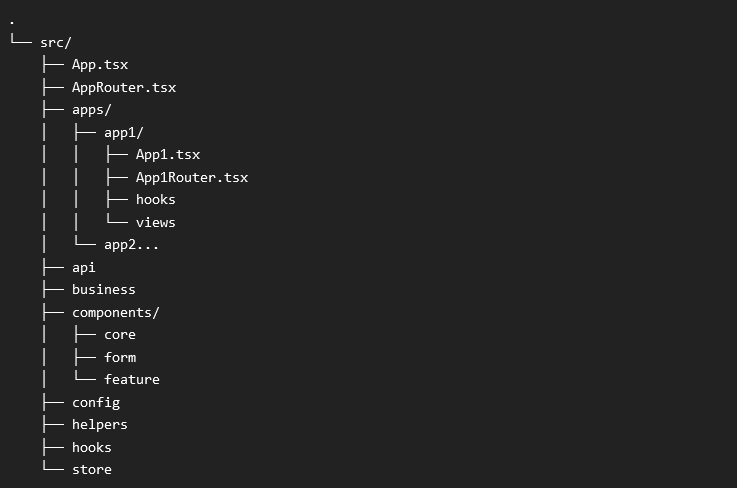
\includegraphics[scale=0.5]{figures/web Concept/struct.png}}
		\caption{Directory Structure}
		\label{dir_str}
	\end{center}
\end{figure}
Therefore we can understand the proposed directory structure with the help of Figure \ref{dir_str} and the actual directory structure \hyperlink{mylink}{as shown here}.

\newpage

\subsection{Physical}
The deployment of our system is presented in the figure below:
\begin{figure}[H]
	\begin{center}
		{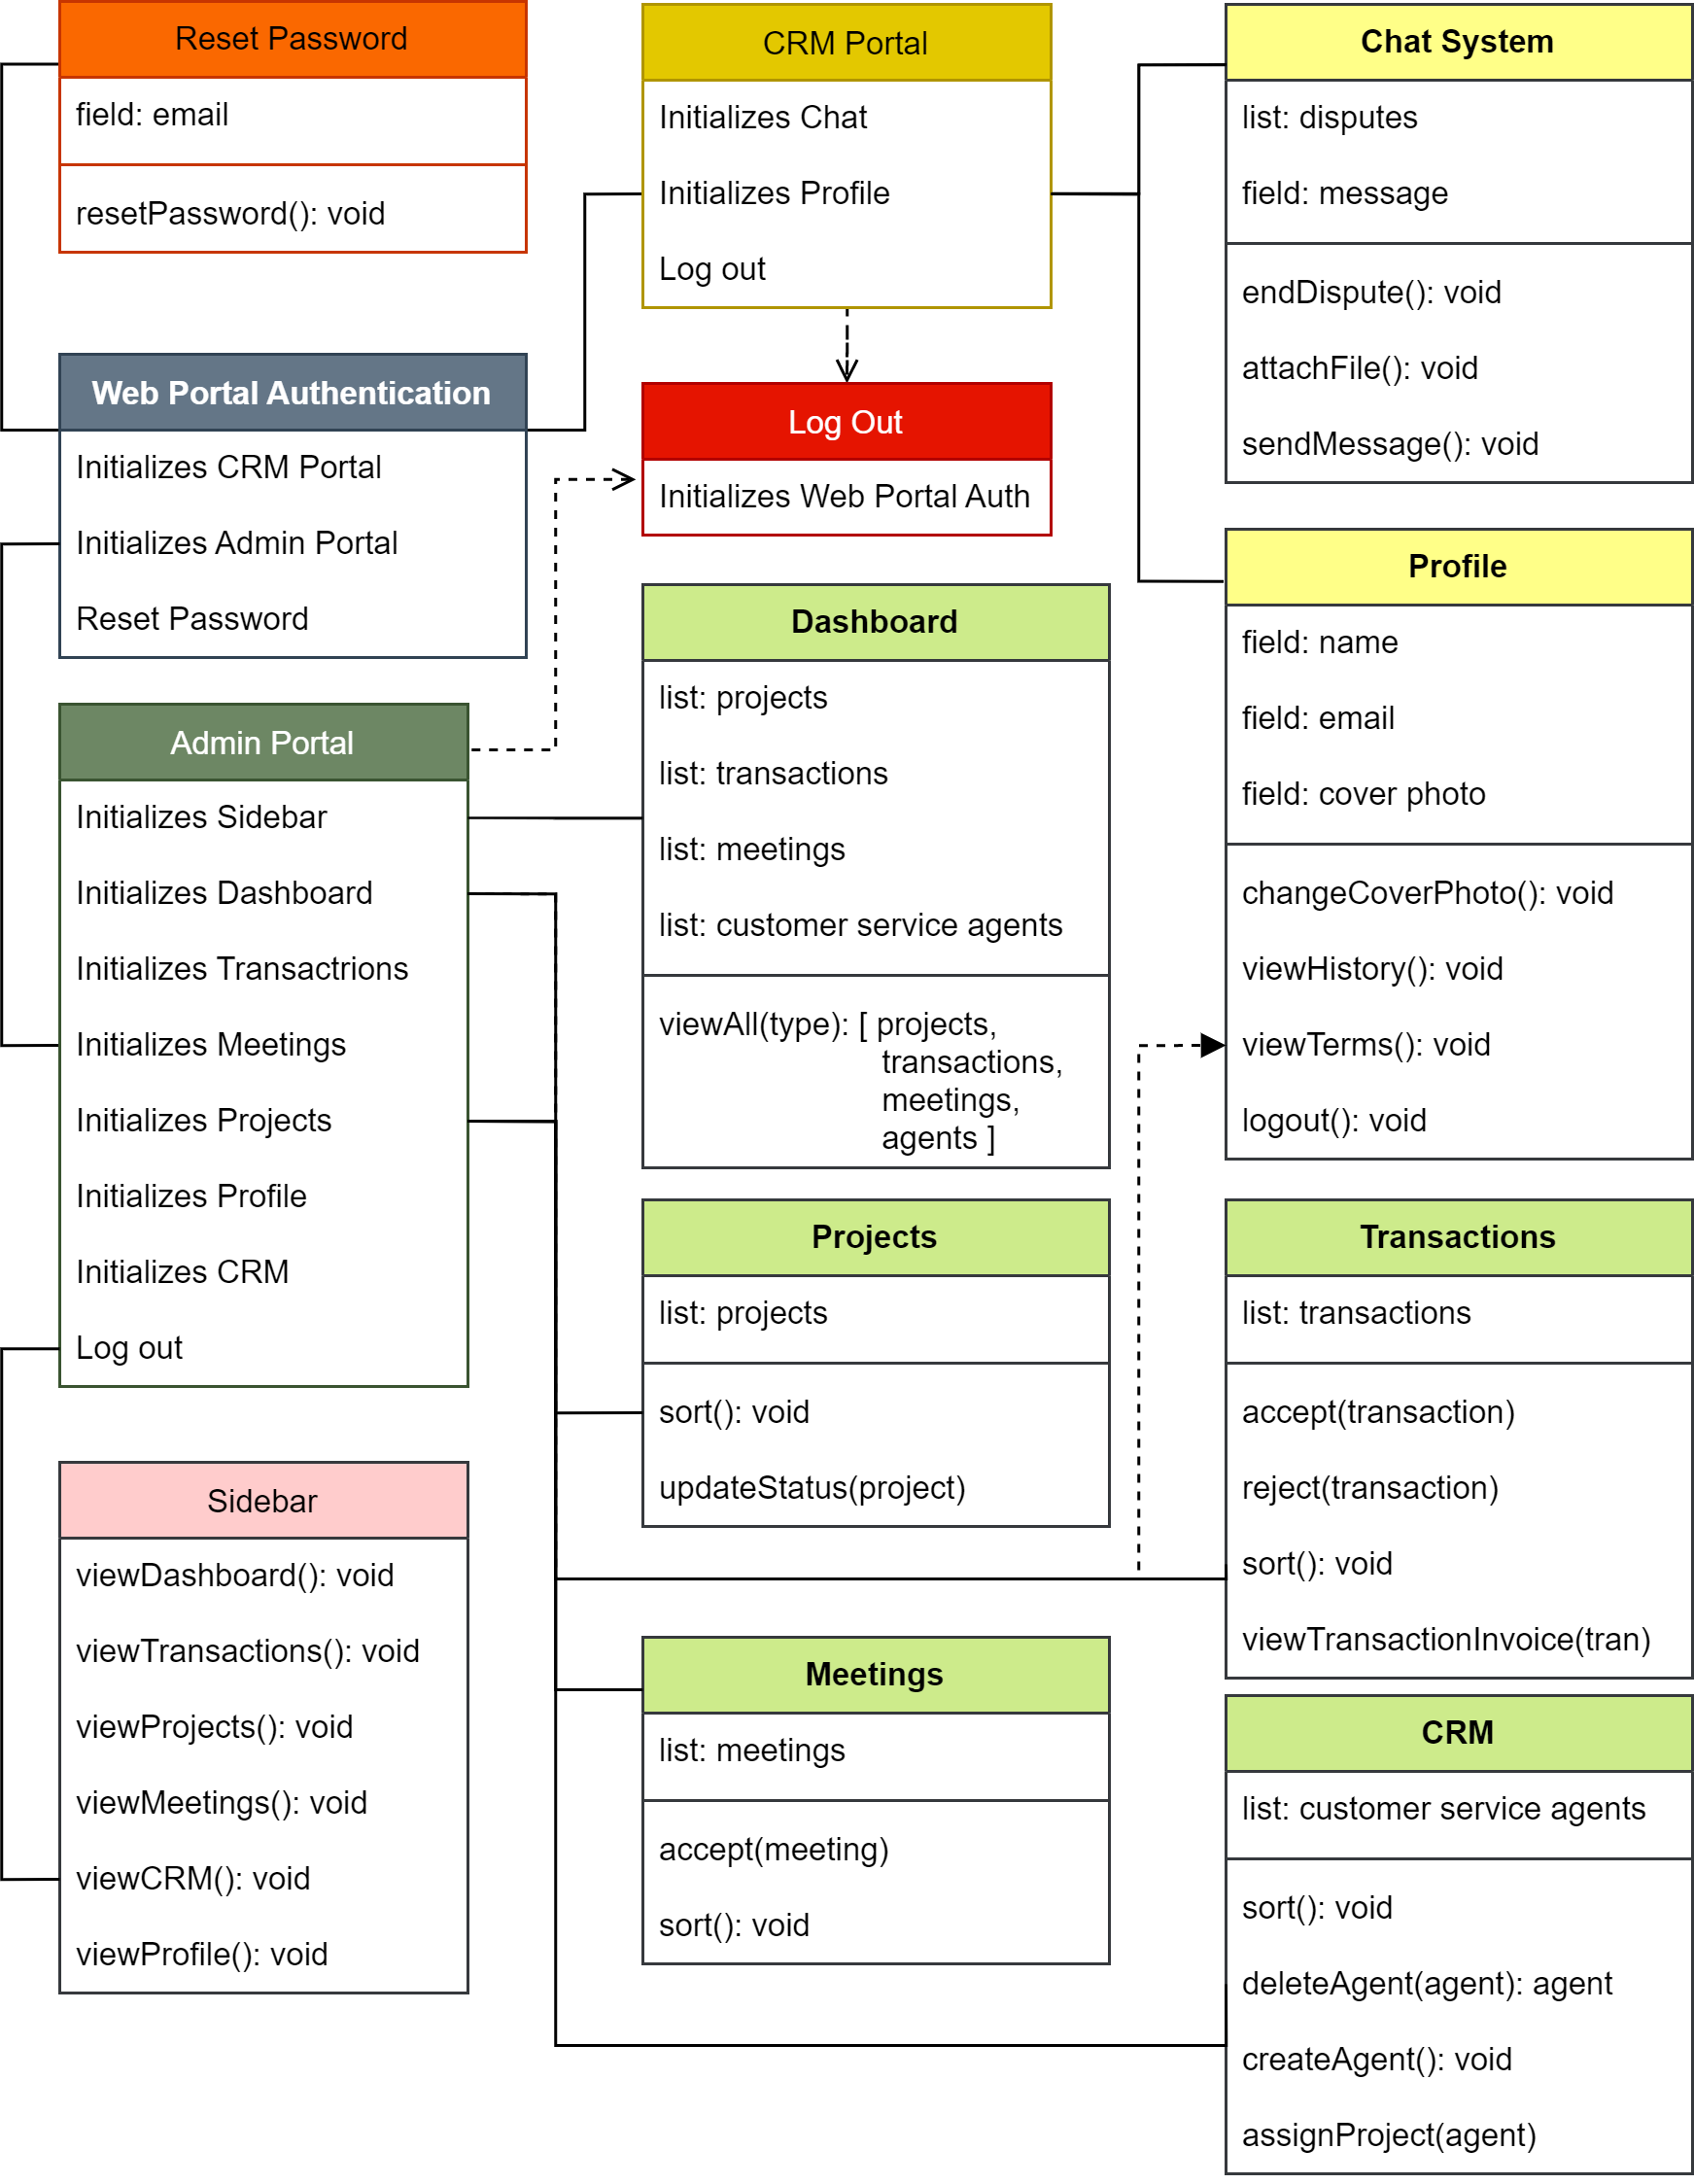
\includegraphics[scale=.9]{figures/web Concept/web-deployment (1).png}}
		\caption{Deployment Diagram}
		\label{fig:dep}
	\end{center}
\end{figure}

\subsection{Security}
We have kept in mind the security aspect of the system. For that purpose we are using Sha-256 encryption for password to store in the database. Moreover Web portal authentication is used for the access of Admin and CRM portal. The conceptual diagram is shown in Figure \ref{web_package}.
Where as Client can view the mobile app in guest mode for the tour of our application. As shown in Figure \ref{first_screen}. Owner functionality and Customer functionality is not available in the guest mode. Guest can only view different projects in their role.

\section{Low Level Design}
\subsection{Mobile Authentication}
\begin{figure}[H]
	\begin{center}
		\shadowbox{
\includegraphics[scale=0.6]{figures/mobile/01_Loding screen.png}}
		\caption{Splash Screen}
	\end{center}
\end{figure}
\begin{figure}[H]
	\begin{center}
		\shadowbox{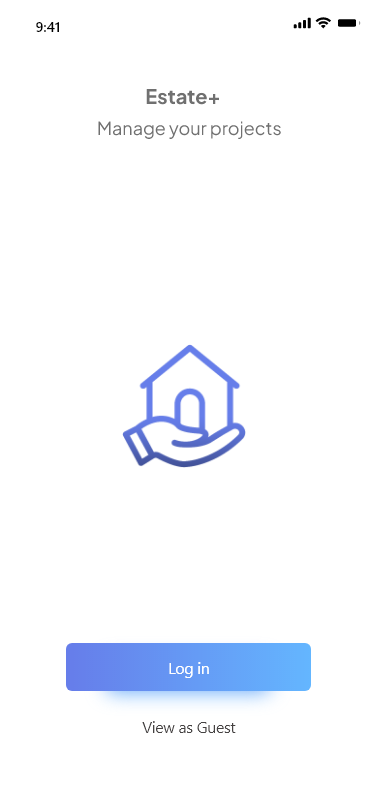
\includegraphics[scale=0.8]{figures/mobile/02_1st Screen.png}}
		\caption{First Screen}
		\label{first_screen}
	\end{center}
\end{figure}
\newpage
\begin{figure}[H]
	\begin{center}
		\shadowbox{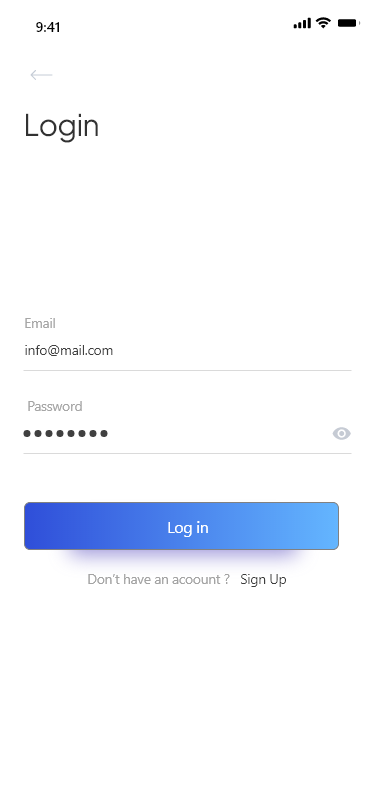
\includegraphics[scale=0.8]{figures/mobile/03_Login Page.png}}
		\caption{Login Screen}
	\end{center}
\end{figure}
\newpage
\begin{figure}[H]
	\begin{center}
		\shadowbox{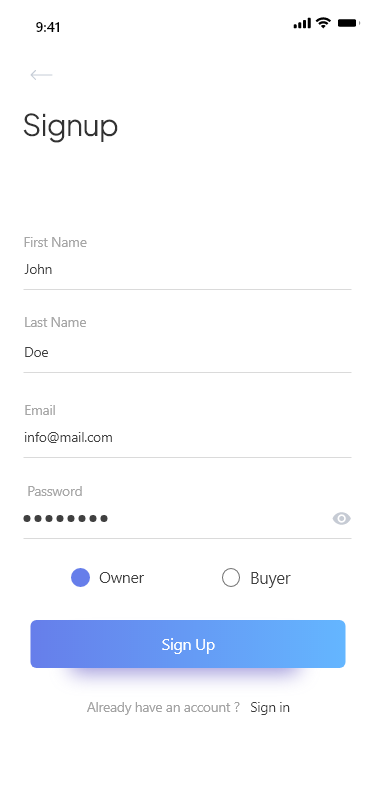
\includegraphics[scale=0.8]{figures/mobile/04_Sign Up.png}}
		\caption{Sign up Screen}
	\end{center}
\end{figure}
\subsection{Client View} \label{client_view}
\begin{figure}[H]
	\begin{center}
		\shadowbox{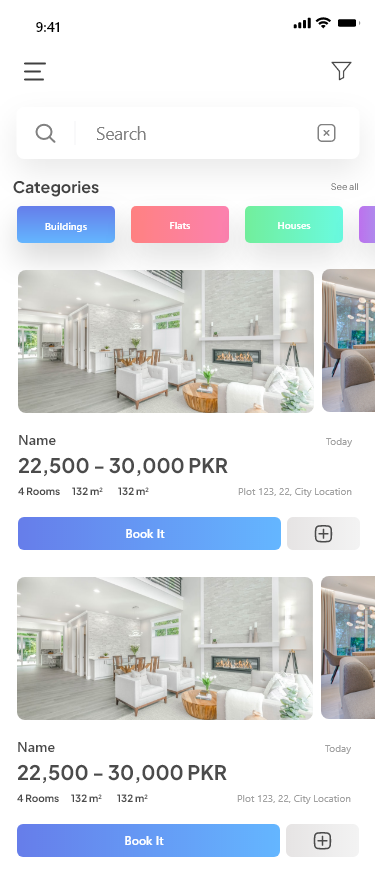
\includegraphics[scale=0.6]{figures/mobile/05_Client_Home.png}}
		\caption{Client Home}
	\end{center}
\end{figure}
\newpage
\begin{figure}[H]
	\begin{center}
		\shadowbox{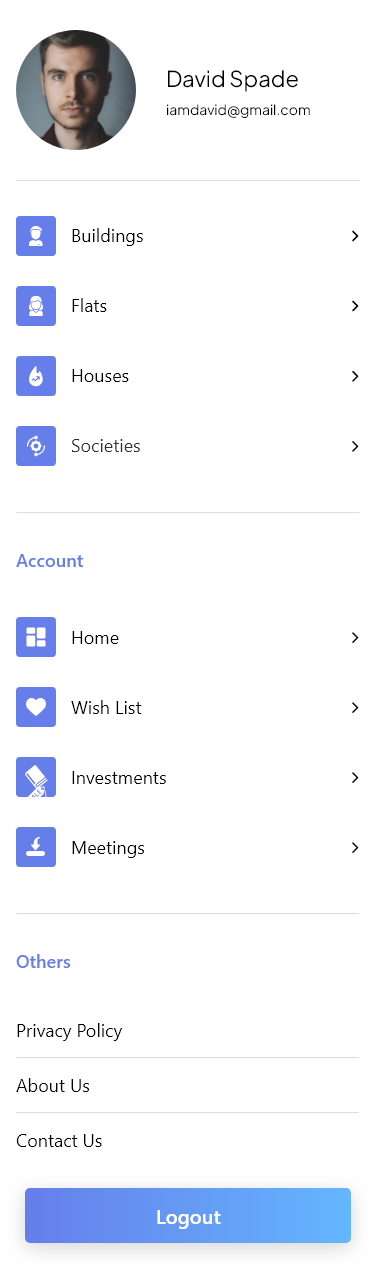
\includegraphics[scale=0.5]{figures/mobile/06_Drawer.png}}
		\caption{Client Drawer}
	\end{center}
\end{figure}
\newpage
\begin{figure}[H]
	\begin{center}
		\shadowbox{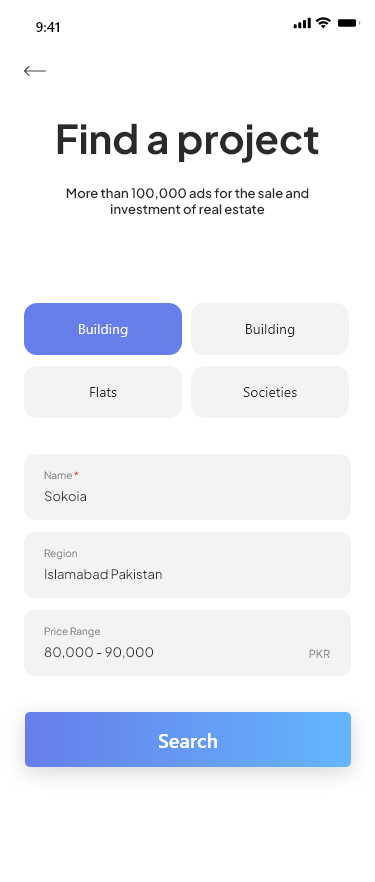
\includegraphics[scale=0.8]{figures/mobile/07_Search.png}}
		\caption{Search Screen}
	\end{center}
\end{figure}
\newpage
\begin{figure}[H]
	\begin{center}
		\shadowbox{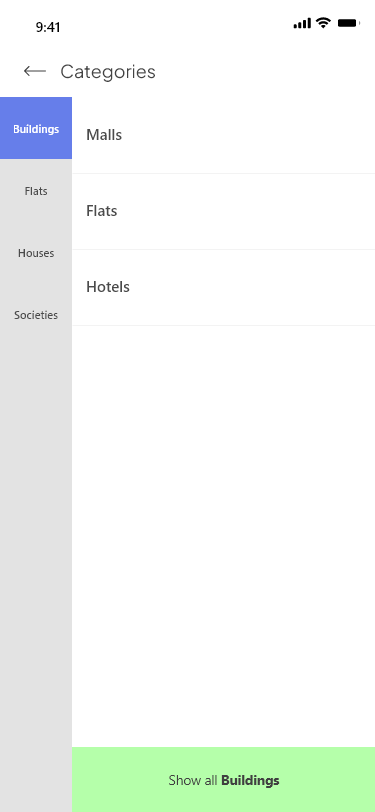
\includegraphics[scale=0.8]{figures/mobile/08_Categories.png}}
		\caption{Categories}
	\end{center}
\end{figure}
\newpage
\newpage
\begin{figure}[H]
	\begin{center}
		\shadowbox{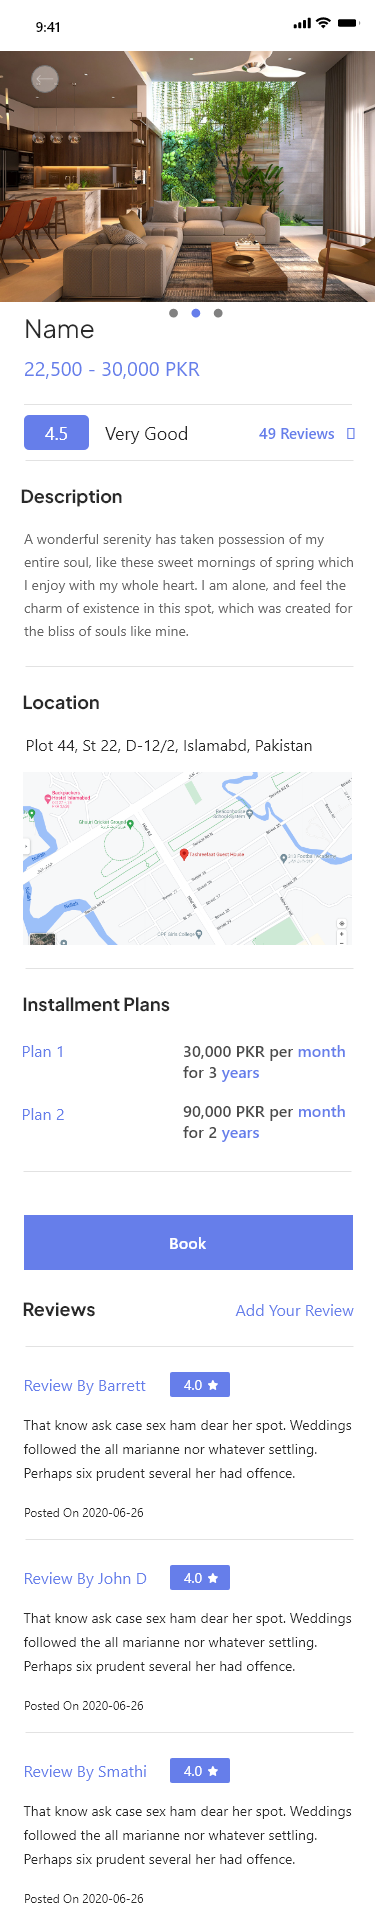
\includegraphics[scale=0.35]{figures/mobile/10_Project_Details.png}}
		\caption{Client Project Details}
	\end{center}
\end{figure}
\newpage
\begin{figure}[H]
	\begin{center}
		\shadowbox{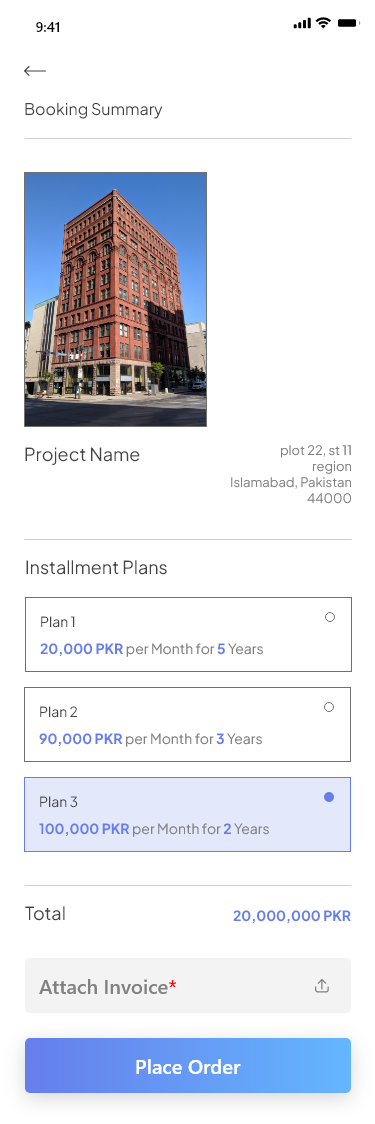
\includegraphics[scale=0.6]{figures/mobile/11_Book Project.png}}
		\caption{Book Project}
	\end{center}
\end{figure}
\newpage
\begin{figure}[H]
	\begin{center}
		\shadowbox{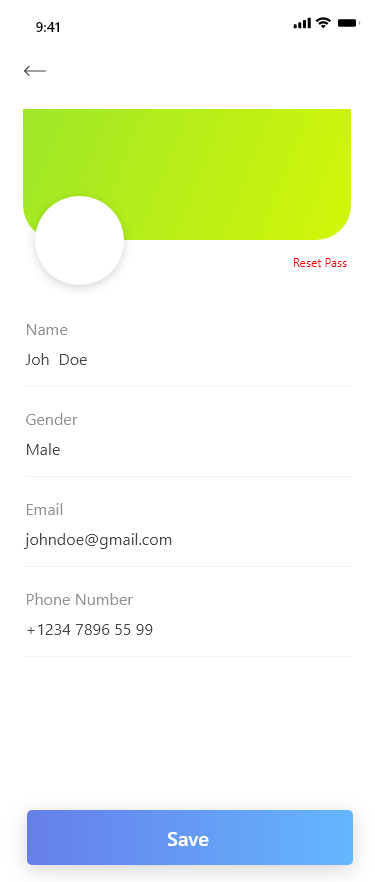
\includegraphics[scale=0.8]{figures/mobile/12_Profile.png}}
		\caption{Client Profile}
	\end{center}
\end{figure}
\newpage
\begin{figure}[H]
	\begin{center}
		\shadowbox{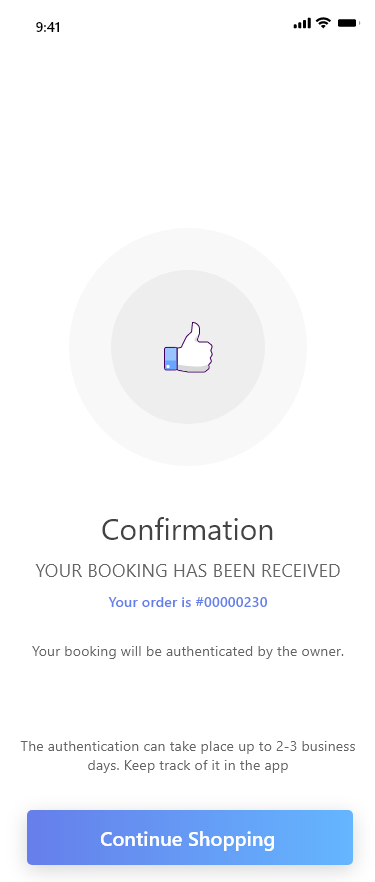
\includegraphics[scale=0.8]{figures/mobile/13_Confirmation.png}}
		\caption{Confirmation}
	\end{center}
\end{figure}
\newpage
\begin{figure}[H]
	\begin{center}
		\shadowbox{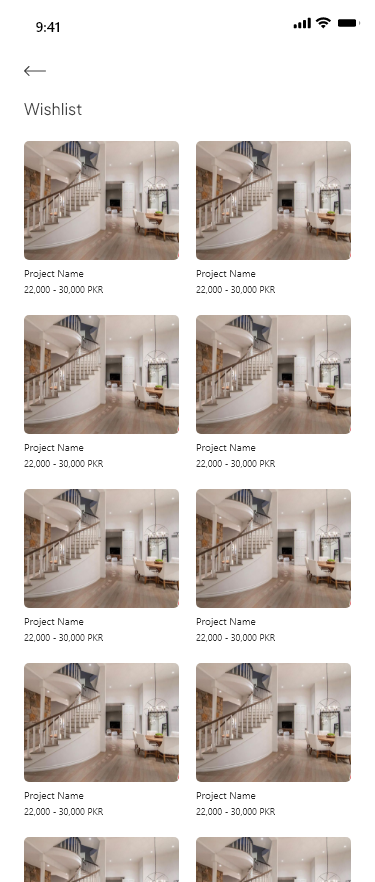
\includegraphics[scale=0.8]{figures/mobile/14_Wishlist.png}}
		\caption{Wish list}
	\end{center}
\end{figure}
\newpage
\begin{figure}[H]
	\begin{center}
		\shadowbox{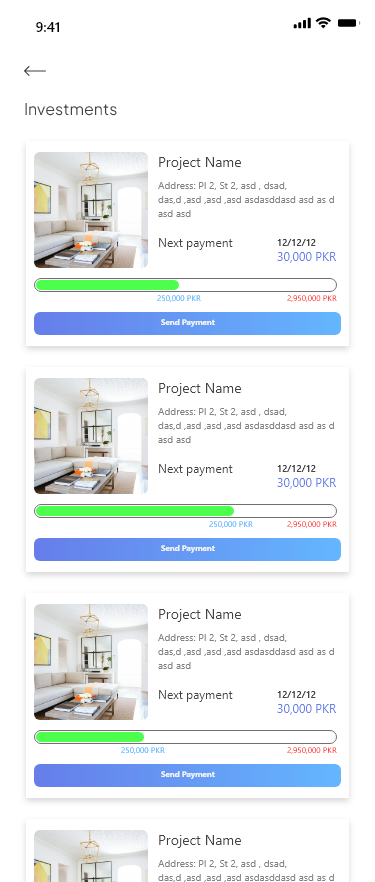
\includegraphics[scale=0.8]{figures/mobile/15_Investments.png}}
		\caption{Investments}
	\end{center}
\end{figure}
\newpage
\begin{figure}[H]
	\begin{center}
		\shadowbox{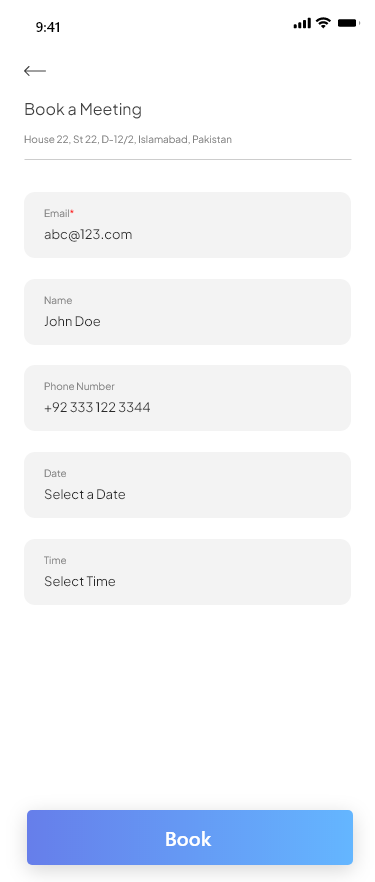
\includegraphics[scale=0.8]{figures/mobile/16_Book Meeting.png}}
		\caption{Book Meeting}
	\end{center}
\end{figure}
\newpage
\begin{figure}[H]
	\begin{center}
		\shadowbox{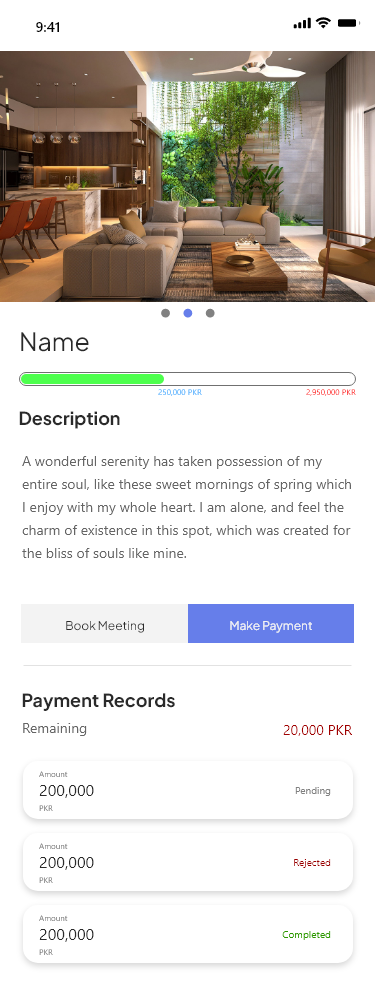
\includegraphics[scale=0.6]{figures/mobile/17_Investment_Detail.png}}
		\caption{Investment Detail}
	\end{center}
\end{figure}
\newpage
\begin{figure}[H]
	\begin{center}
		\shadowbox{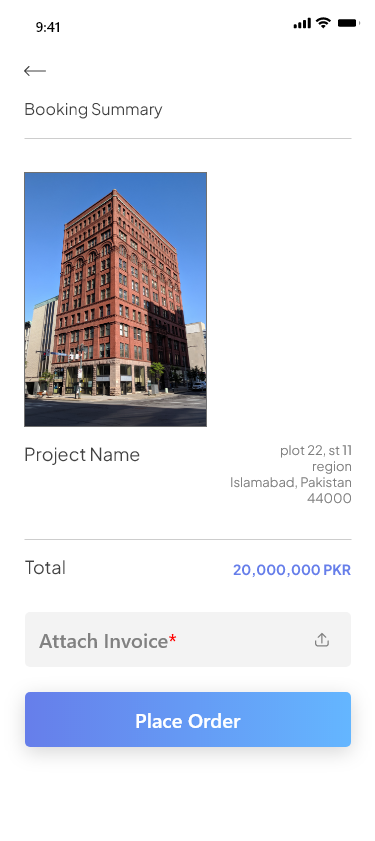
\includegraphics[scale=0.8]{figures/mobile/18_Payment.png}}
		\caption{Payment}
	\end{center}
\end{figure}
\newpage
\subsection{Owner View}
\begin{figure}[H]
	\begin{center}
		\shadowbox{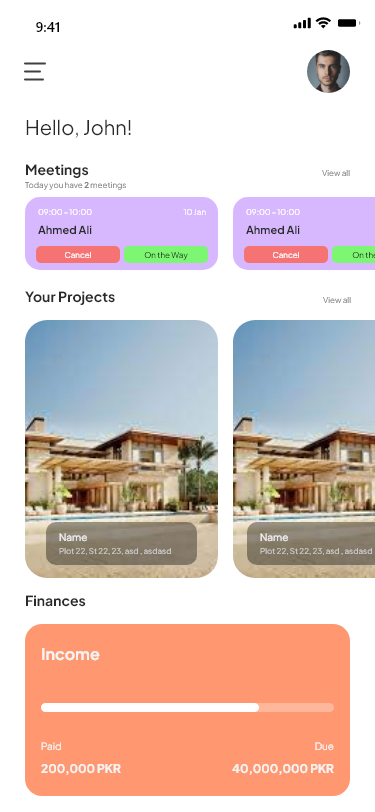
\includegraphics[scale=0.7]{figures/mobile/19_Owner_Home.png}}
		\caption{Owner Home}
	\end{center}
\end{figure}
\newpage
\begin{figure}[H]
	\begin{center}
		\shadowbox{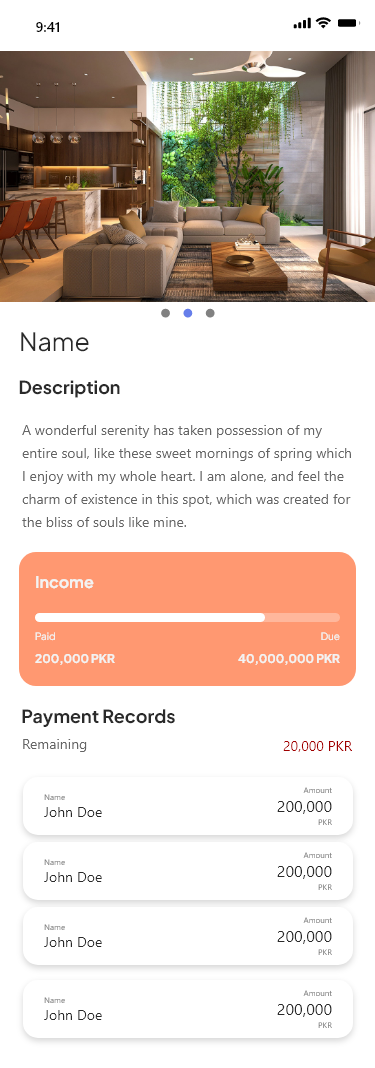
\includegraphics[scale=0.6]{figures/mobile/20_Project.png}}
		\caption{Owner Project Details}
	\end{center}
\end{figure}
\newpage
\begin{figure}[H]
	\begin{center}
		\shadowbox{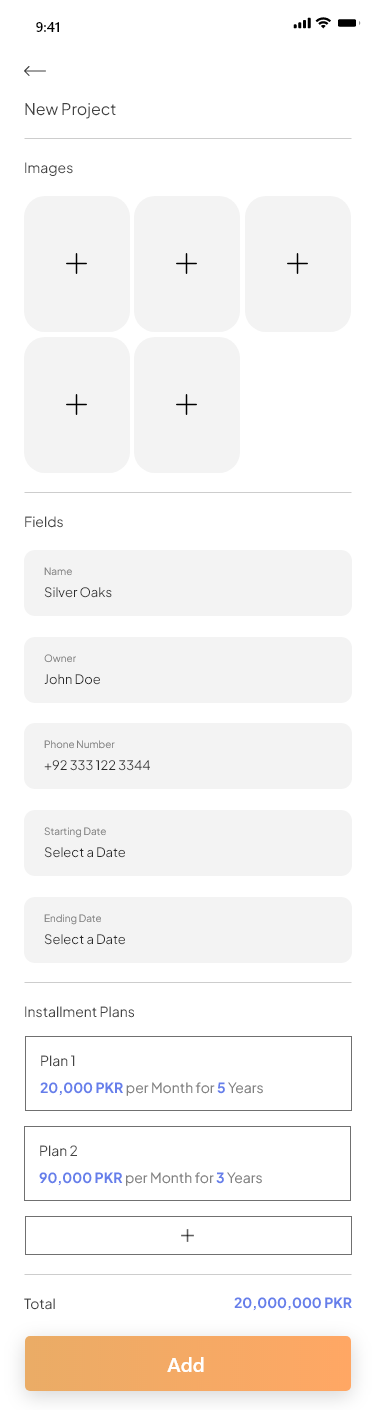
\includegraphics[scale=0.5]{figures/mobile/21_New Project.png}}
		\caption{New Project}
	\end{center}
\end{figure}
\begin{figure}[H]
	\begin{center}
		\shadowbox{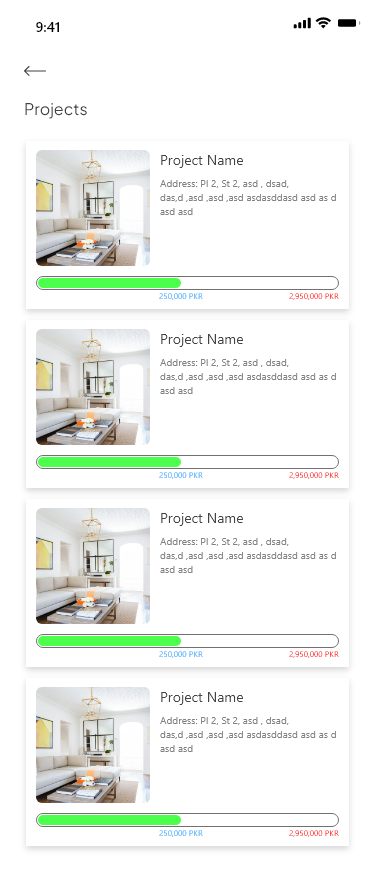
\includegraphics[scale=0.8]{figures/mobile/22_Projects.png}}
		\caption{Owner Project}
	\end{center}
\end{figure}
\newpage
\begin{figure}[H]
	\begin{center}
		\shadowbox{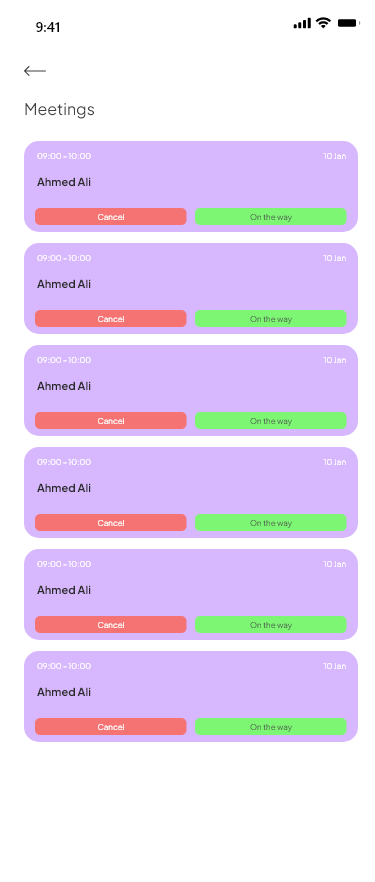
\includegraphics[scale=0.8]{figures/mobile/23_Meetings.png}}
		\caption{Owner Meetings}
	\end{center}
\end{figure}
\newpage
\begin{figure}[H]
	\begin{center}
		\shadowbox{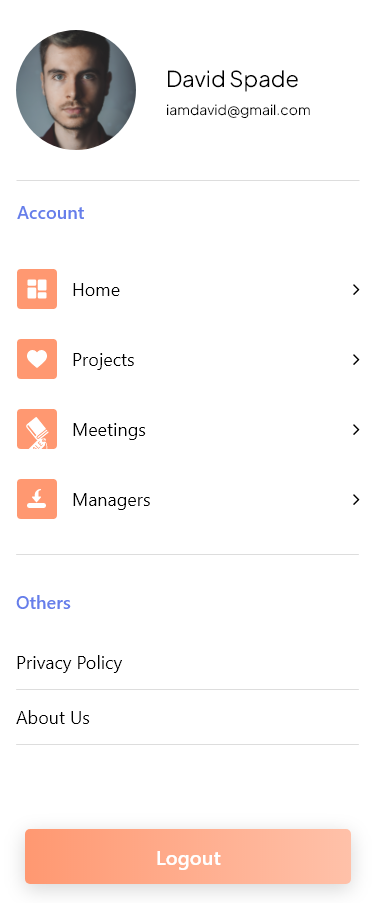
\includegraphics[scale=0.7]{figures/mobile/24_Owner Drawer.png}}
		\caption{Owner Drawer}
	\end{center}
\end{figure}
\newpage
\begin{figure}[H]
	\begin{center}
		\shadowbox{\includegraphics[scale=0.8]{figures/mobile/25_Confirmation – 1.png}}
		\caption{Confirmation}
	\end{center}
\end{figure}
\newpage
\begin{figure}[H]
	\begin{center}
		\shadowbox{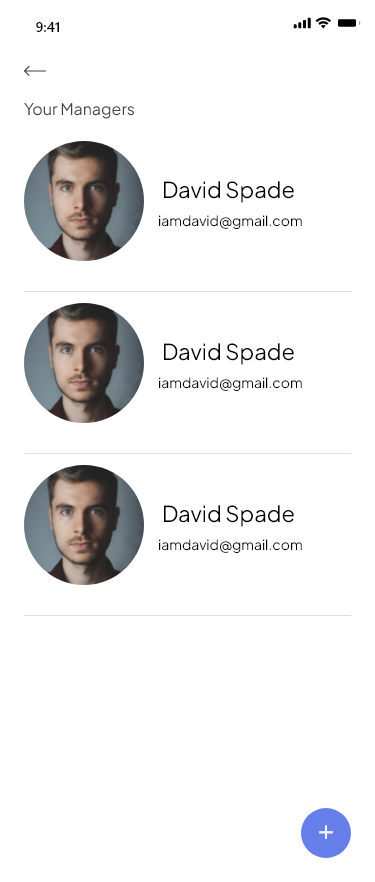
\includegraphics[scale=0.8]{figures/mobile/26_Managers.png}}
		\caption{Managers}
	\end{center}
\end{figure}
\newpage
\begin{figure}[H]
	\begin{center}
		\shadowbox{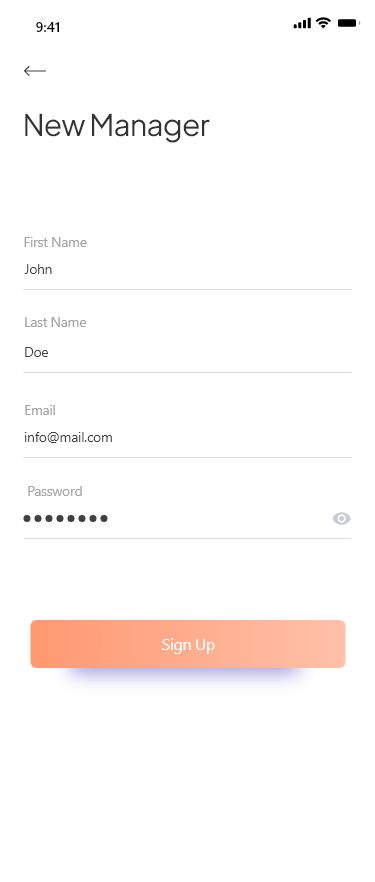
\includegraphics[scale=0.8]{figures/mobile/27_New Manager.png}}
		\caption{New Manager}
	\end{center}
\end{figure}
\newpage
\subsection{CRM for Client}
\begin{figure}[H]
	\begin{center}
		\shadowbox{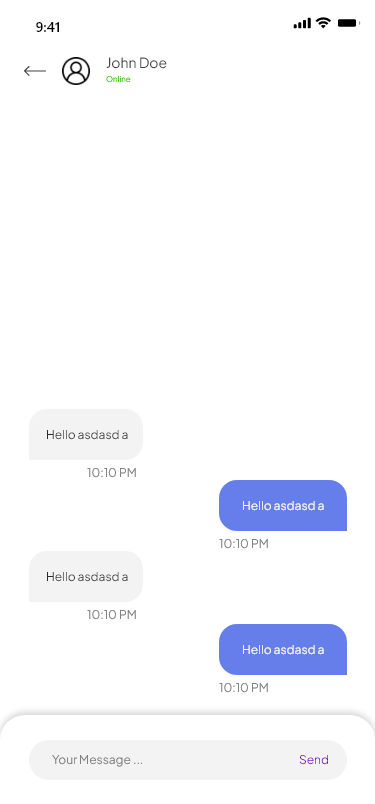
\includegraphics[scale=0.7]{figures/mobile/09_CRM.png}}
		\caption{Contact Us}
		\label{fig:crm_client}
	\end{center}
\end{figure}
\newpage
\subsection{Complaint Management System for Client}
\begin{figure}[H]
	\begin{center}
		\shadowbox{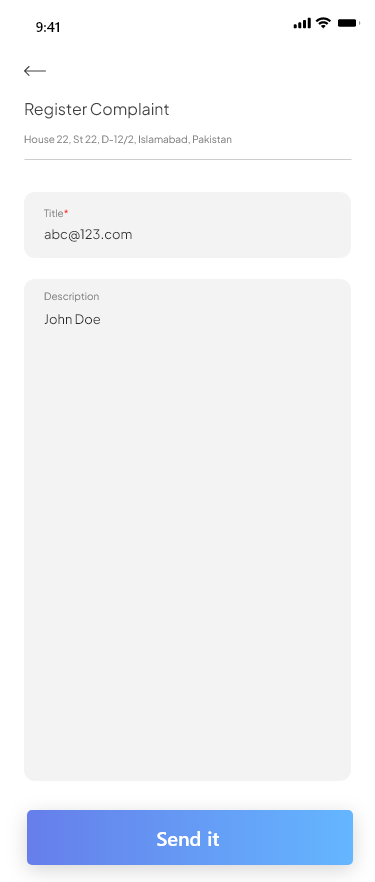
\includegraphics[scale=0.6]{figures/mobile/28_Register Complaint.png}}
		\caption{Register Complaint}
		\label{fig:cpm_register_user}
	\end{center}
\end{figure}
\newpage
\begin{figure}[H]
	\begin{center}
		\shadowbox{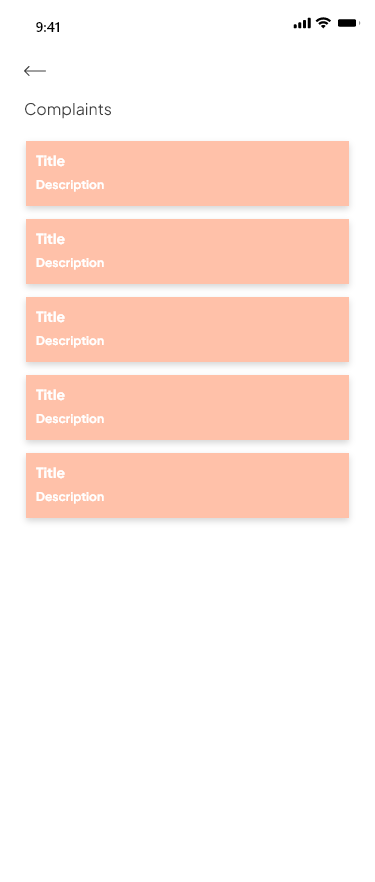
\includegraphics[scale=0.8]{figures/mobile/29_Complaints.png}}
		\caption{All Complaints}
		\label{fig:cpm_detail_user}
	\end{center}
\end{figure}
\begin{figure}[H]
	\begin{center}
		\shadowbox{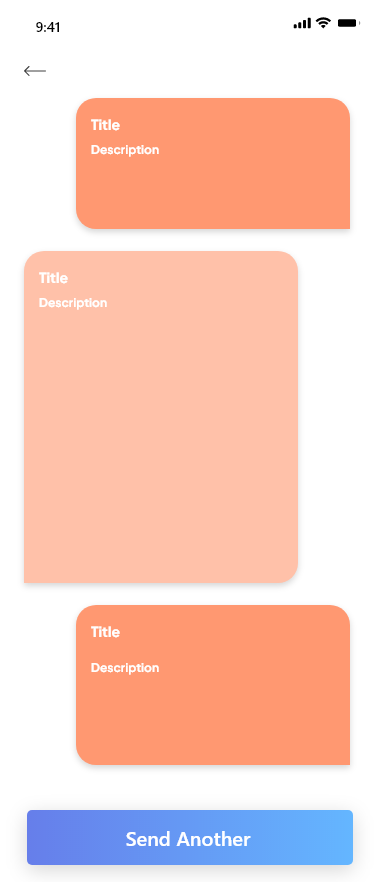
\includegraphics[scale=0.8]{figures/mobile/30_Complaint Detail.png}}
		\caption{Complaint Detail}
		\label{fig:cpm_detail_user}
	\end{center}
\end{figure}
\newpage
\subsection{Web Authentication}
\begin{figure}[H]
	\begin{center}
		\shadowbox{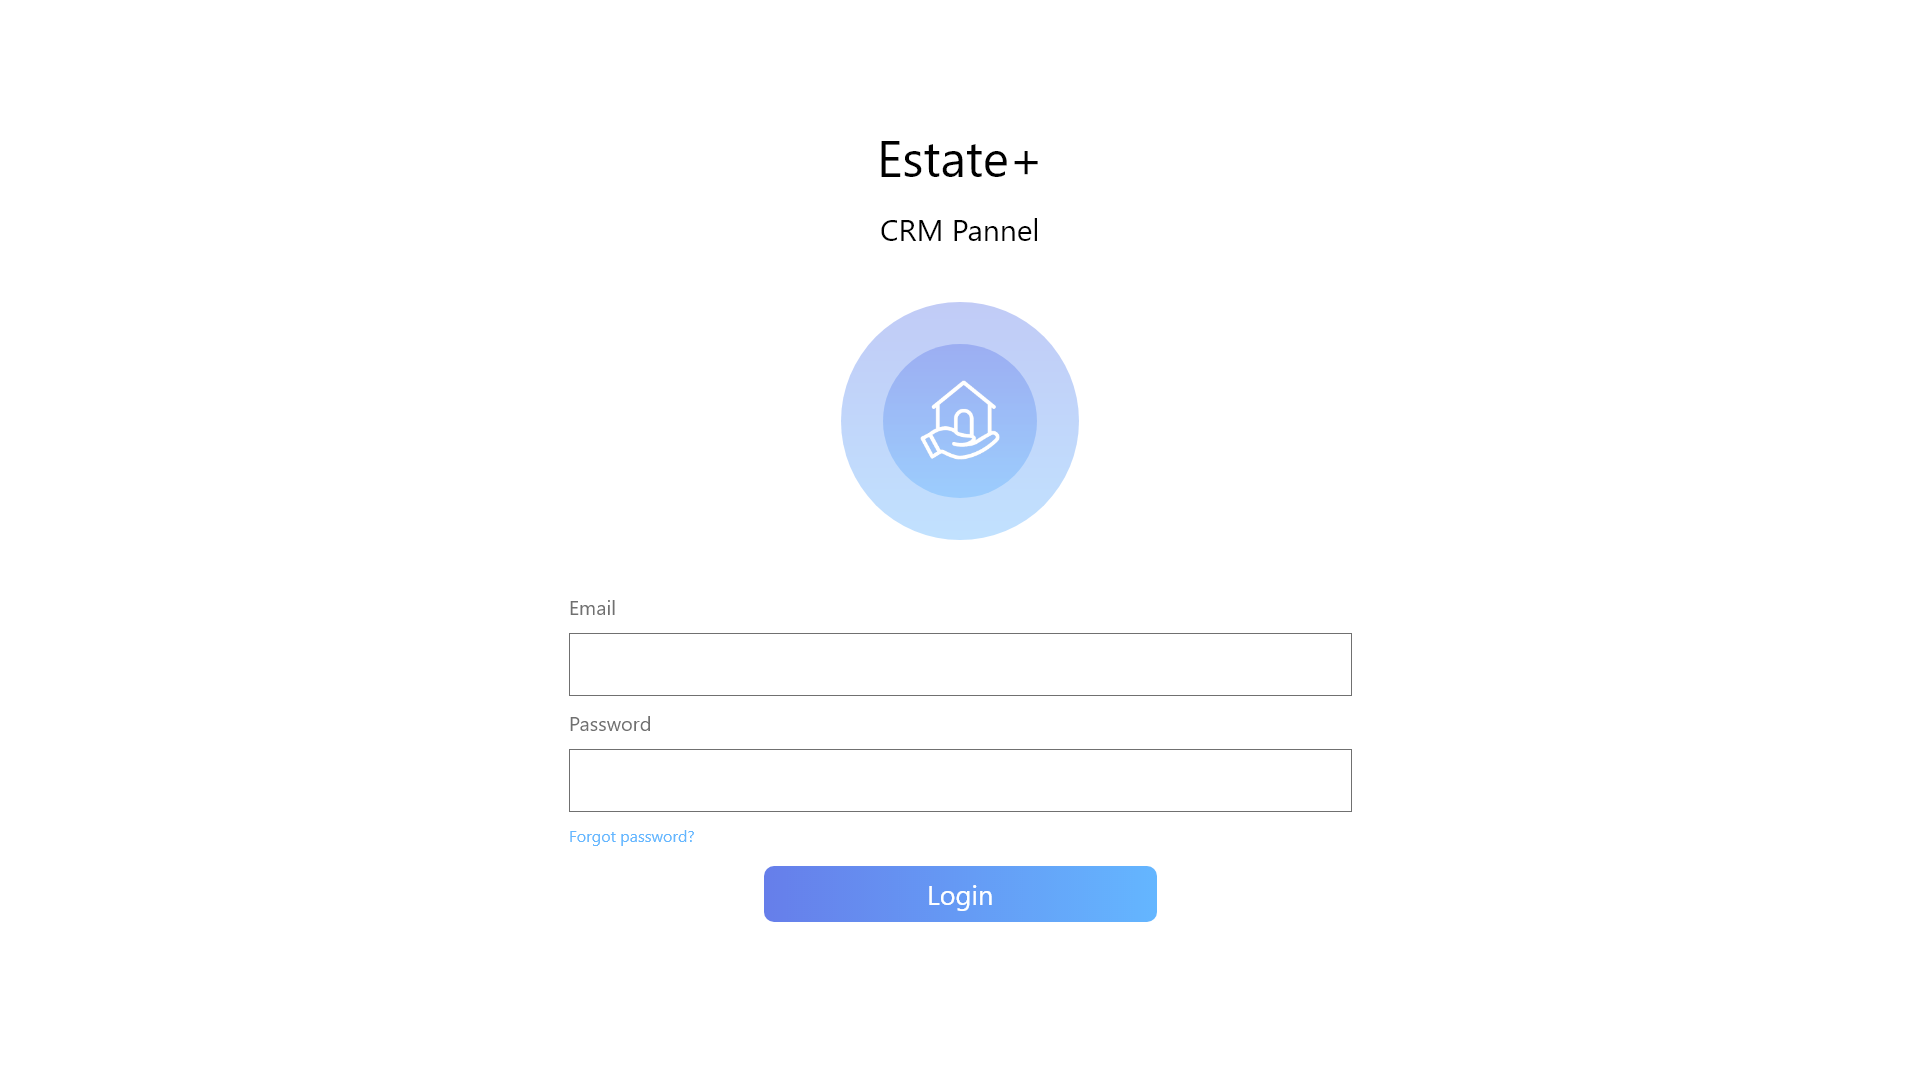
\includegraphics[scale=0.2]{figures/web/01_Login.png}}
		\caption{Web Login}
	\end{center}
\end{figure}
\begin{figure}[H]
	\begin{center}
		\shadowbox{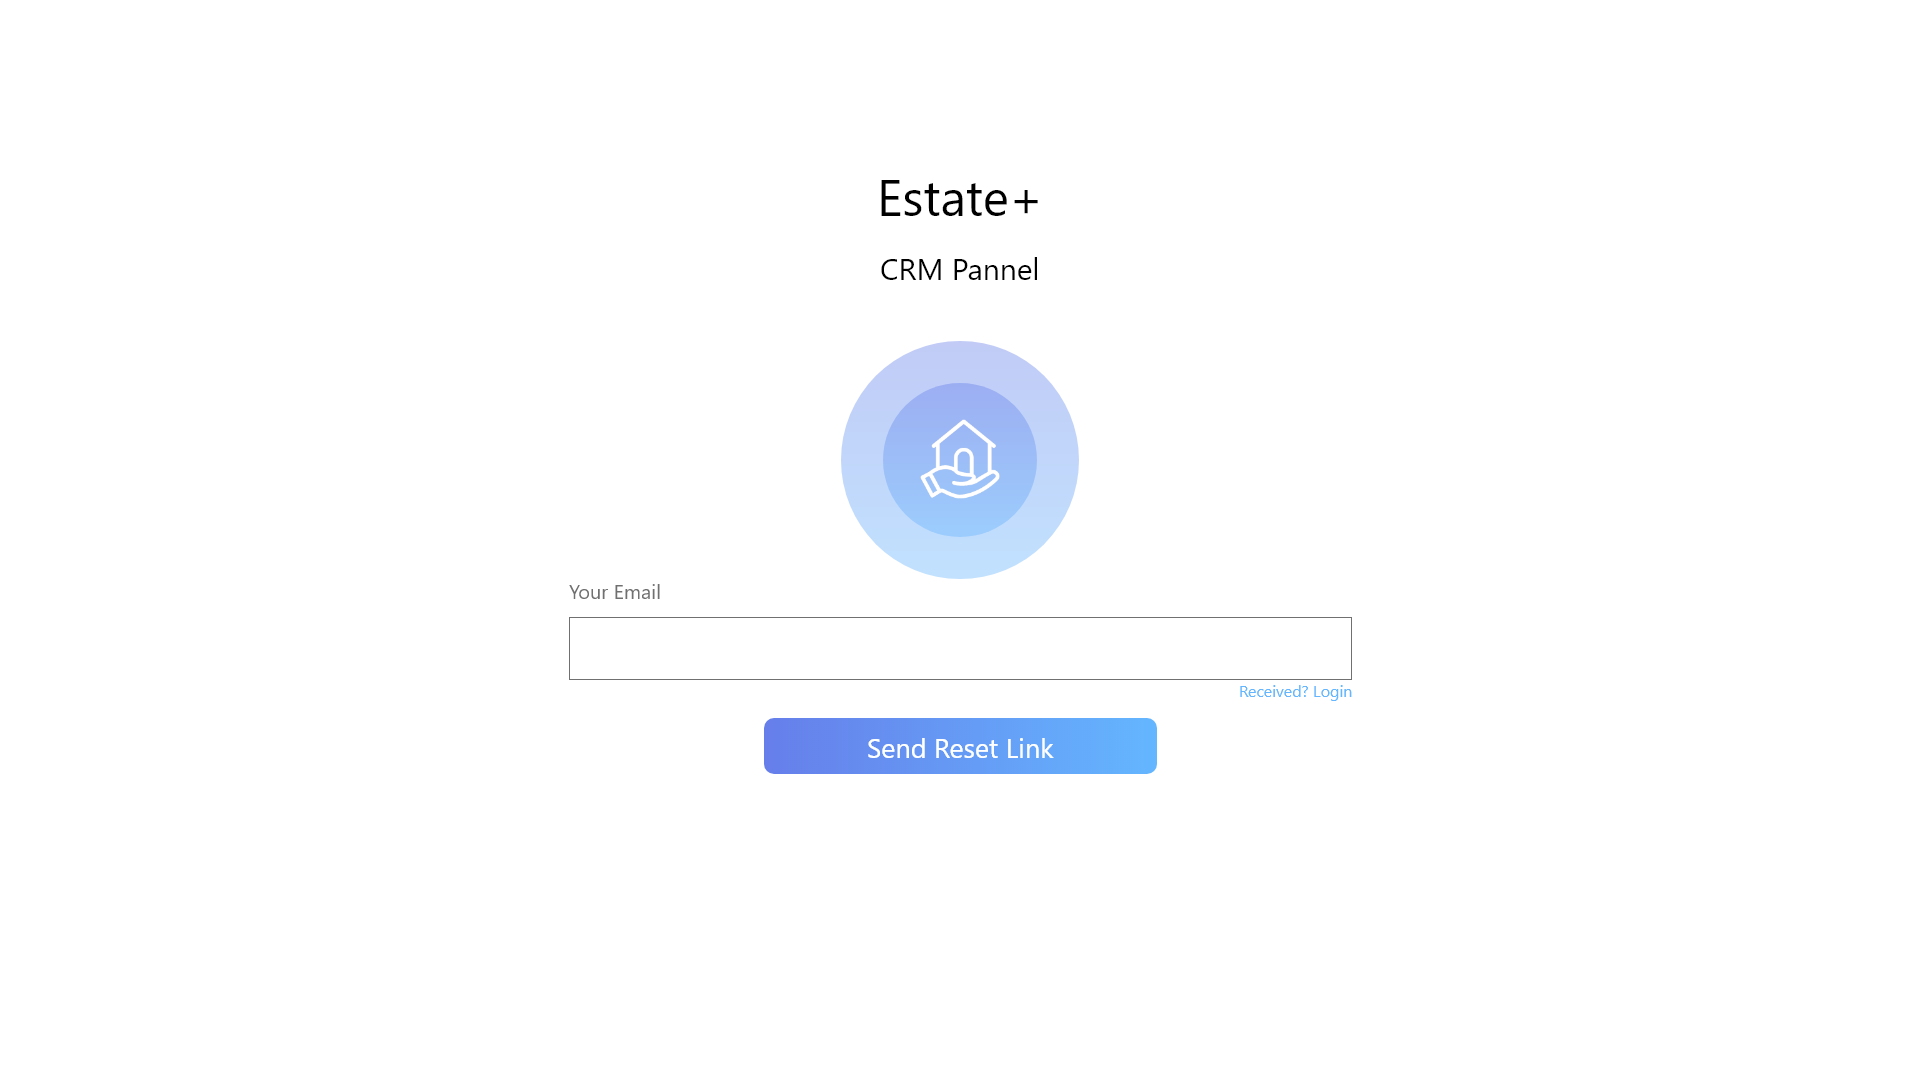
\includegraphics[scale=0.24]{figures/web/02_Forgot Password.png}}
		\caption{Forgot Password}
	\end{center}
\end{figure}
\begin{figure}[H]
	\begin{center}
		\shadowbox{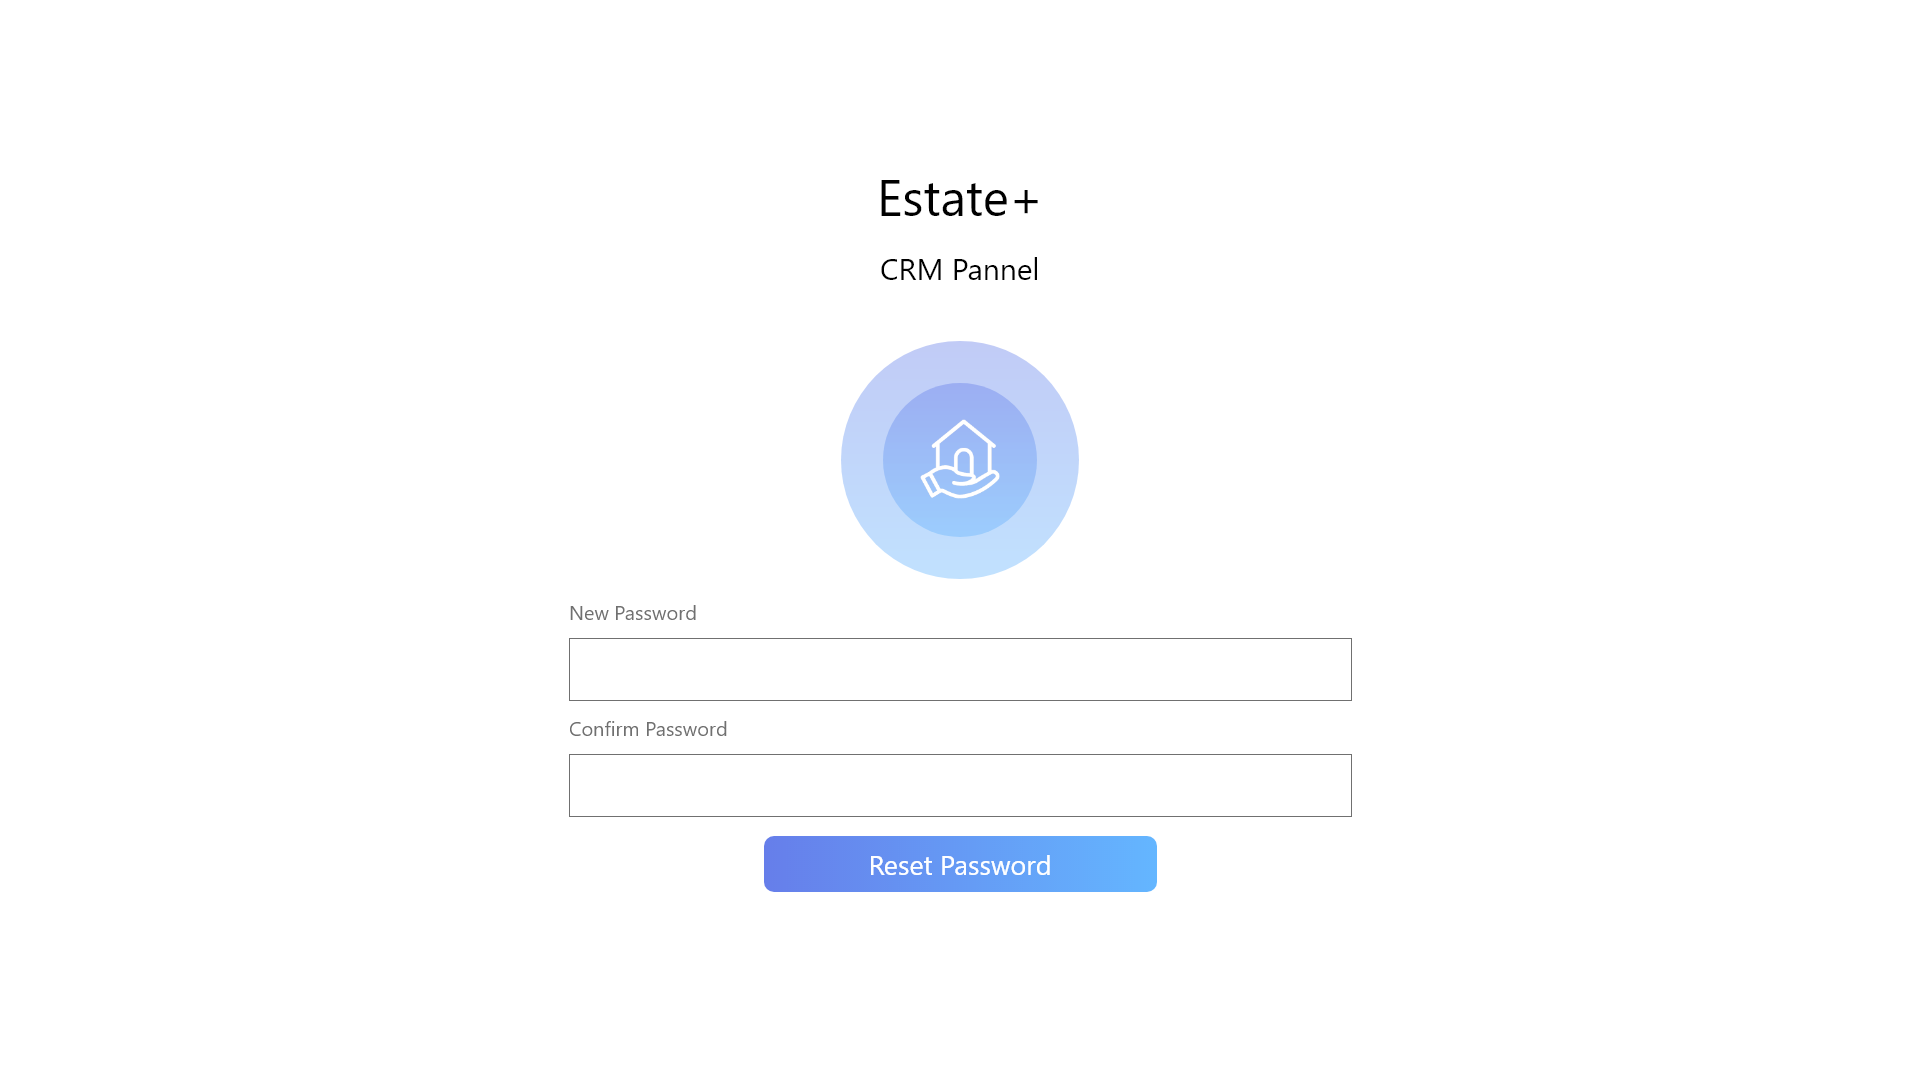
\includegraphics[scale=0.24]{figures/web/03_Reset Password.png}}
		\caption{Reset Password}
	\end{center}
\end{figure}
\newpage
\subsection{CRM for Agent}
\begin{figure}[H]
	\begin{center}
		\shadowbox{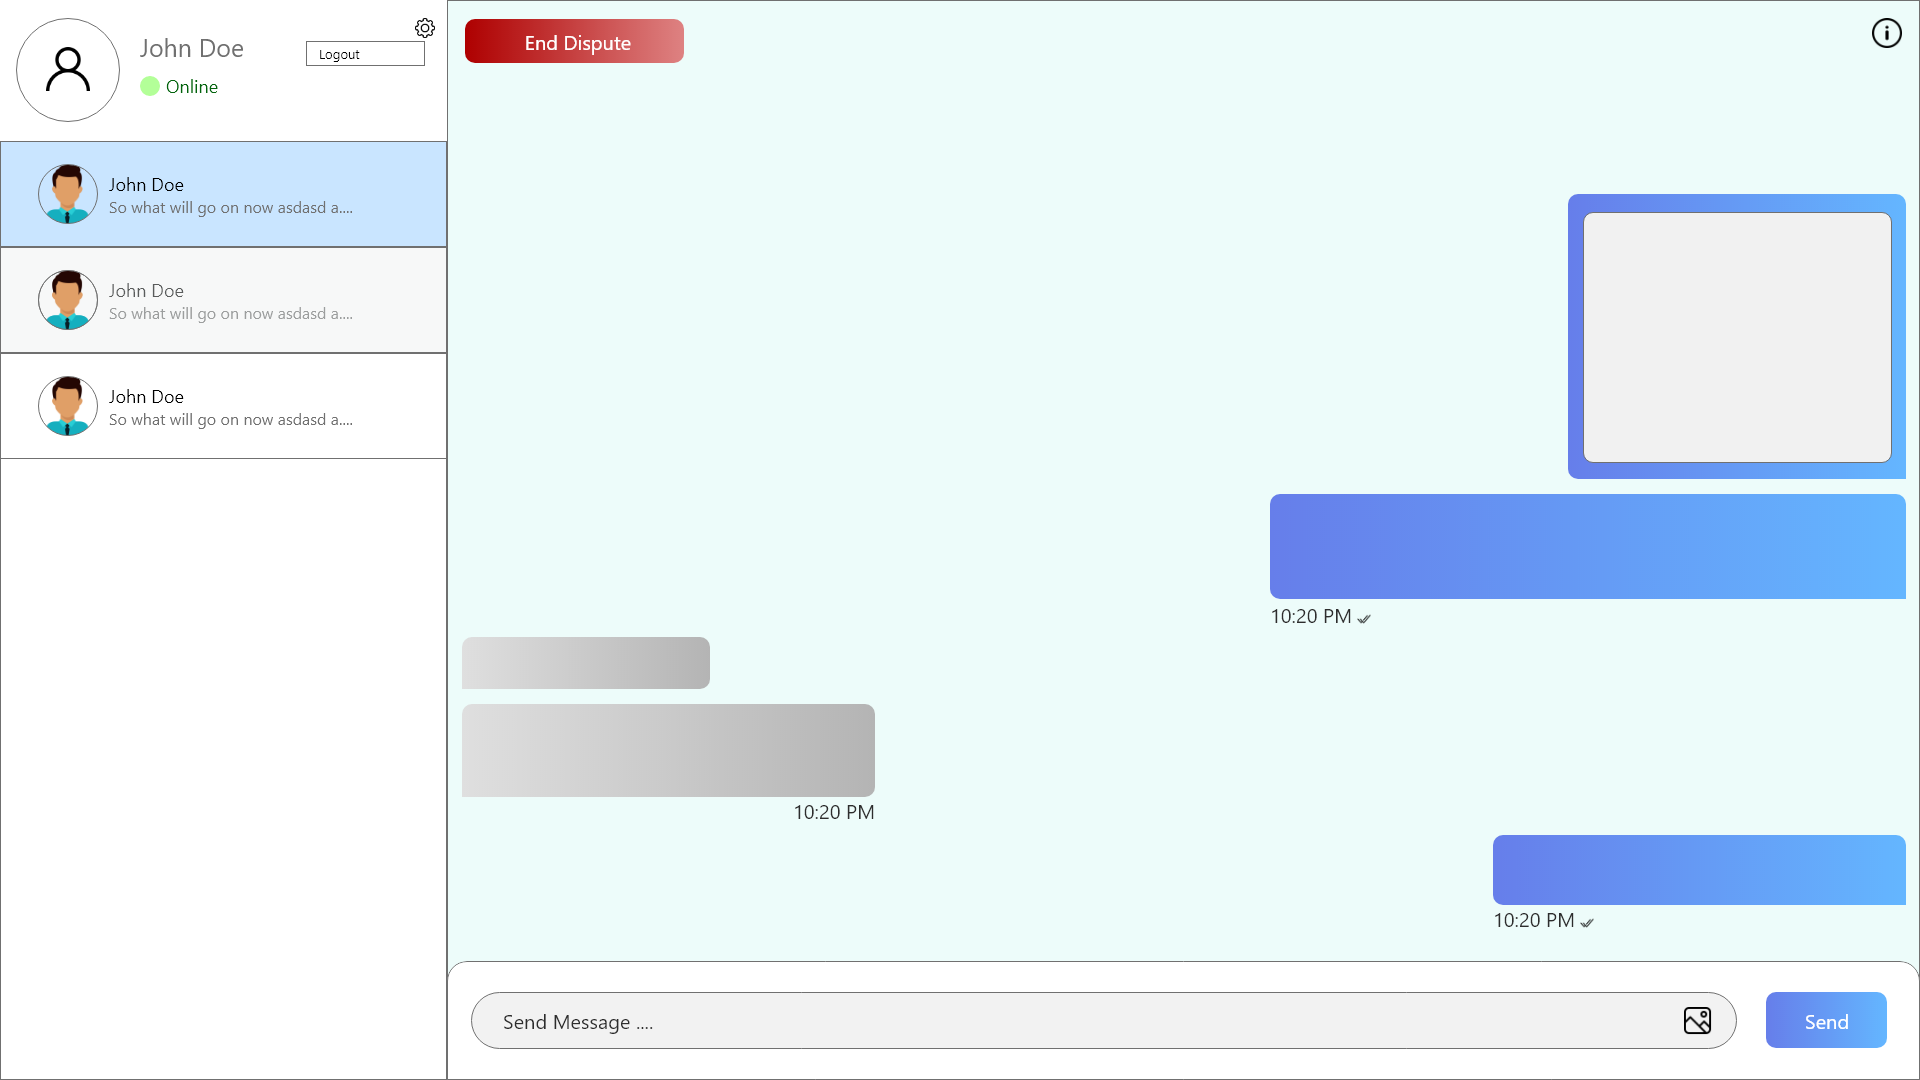
\includegraphics[scale=0.2]{figures/web/4_Chat.png}}
		\caption{CRO Chat}
		\label{fig:crm_agent}
	\end{center}
\end{figure}
\begin{figure}[H]
	\begin{center}
		\shadowbox{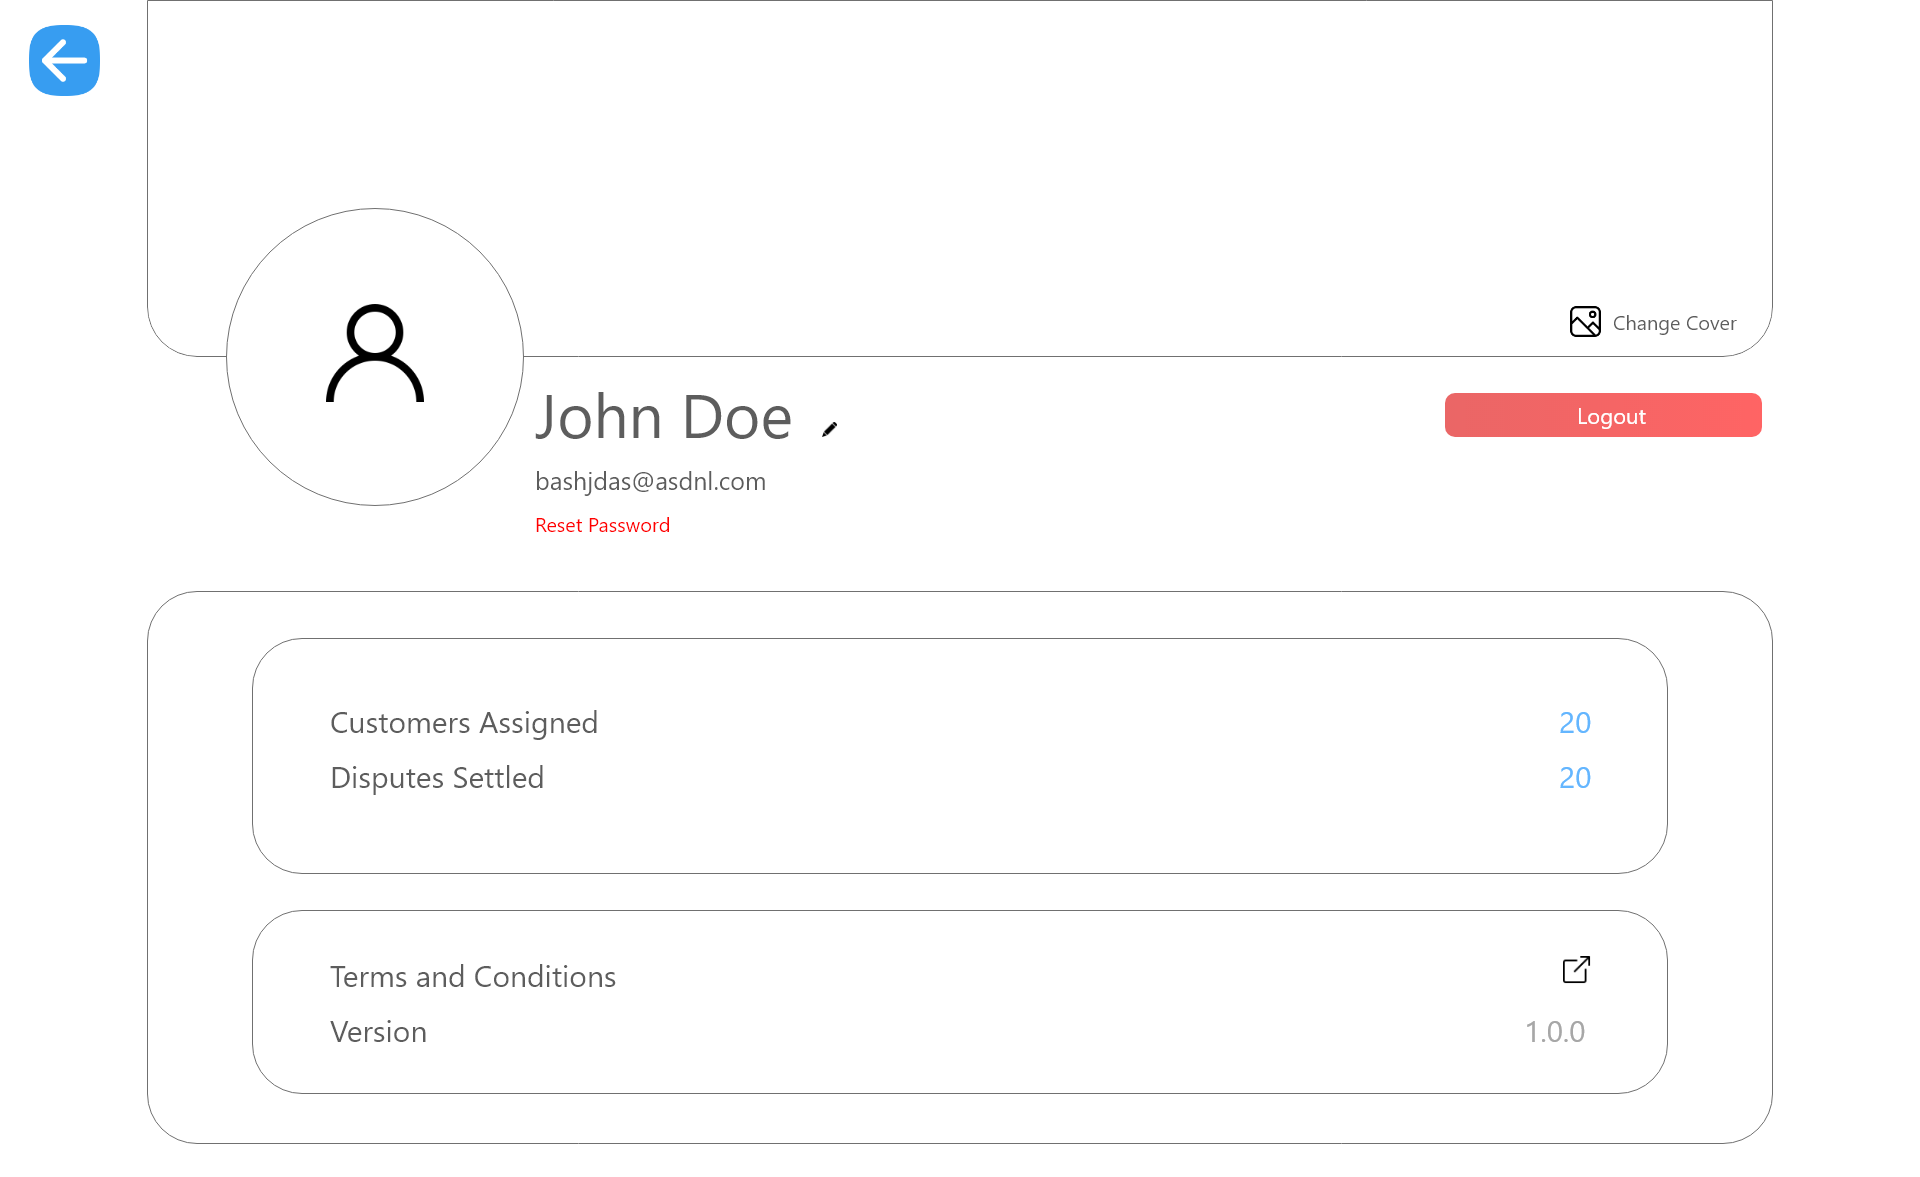
\includegraphics[scale=0.24]{figures/web/05_Profile.png}}
		\caption{CRO Profile}
	\end{center}
\end{figure}
\newpage
\subsection{ERP for Admin}
\begin{figure}[H]
	\begin{center}
		\shadowbox{\includegraphics[scale=0.28]{figures/web_update/web_dash.jpg}}
		\caption{Admin Dashboard}
		\label{manage}
	\end{center}
\end{figure}
\begin{figure}[H]
	\begin{center}
		\shadowbox{\includegraphics[scale=0.3]{figures/web_update/web_dash_hover.jpg}}
		\caption{Admin Dashboard Hover Effect}
	\end{center}
\end{figure}

\begin{figure}[H]
	\begin{center}
		\centering
		\shadowbox{\includegraphics[scale=0.3]{figures/web_update/web_trans.jpg}}
		\caption{Admin Transactions}
	\end{center}
\end{figure}

\begin{figure}[H]
	\begin{center}
		\shadowbox{\includegraphics[scale=0.3]{figures/web_update/web_trans_hover.jpg}}
		\caption{Admin Transactions Hover Effect}
	\end{center}
\end{figure}

\begin{figure}[H]
	\begin{center}
		\shadowbox{\includegraphics[scale=0.3]{figures/web_update/web_trans_modal.jpg}}
		\caption{Admin Transaction Modal}
		\label{create}
	\end{center}
\end{figure}

\begin{figure}[H]
	\begin{center}
		\shadowbox{\includegraphics[scale=0.3]{figures/web_update/web_meet.jpg}}
		\caption{Admin Meetings}
		\label{create}
	\end{center}
\end{figure}

\begin{figure}[H]
	\begin{center}
		\shadowbox{\includegraphics[scale=0.3]{figures/web_update/web_admin_crm.jpg}}
		\caption{Admin CRM Pannel}
		\label{create}
	\end{center}
\end{figure}
\begin{figure}[H]
	\begin{center}
		\shadowbox{\includegraphics[scale=0.3]{figures/web_update/web_admin_crm_modal.jpg}}
		\caption{Admin CRM Pannel Modal}
		\label{create}
	\end{center}
\end{figure}
\begin{figure}[H]
	\begin{center}
		\shadowbox{\includegraphics[scale=0.3]{figures/web_update/web_admin_crm_modal_hover.jpg}}
		\caption{Admin CRM Pannel Modal Hover}
		\label{create}
	\end{center}
\end{figure}


\begin{figure}[H]
	\begin{center}
		\shadowbox{\includegraphics[scale=0.24]{figures/web/11_Profile.png}}
		\caption{Admin Profile}
	\end{center}
\end{figure}
\begin{figure}[H]
	\begin{center}
		\shadowbox{\includegraphics[scale=0.22]{figures/web/14_Complaints.png}}
		\caption{Complaints}
		\label{fig:cpm_admin}
	\end{center}
\end{figure}

\section{GUI Design}
To keep the design simple and easy to understand, certain standard needed to be followed. The standard that was followed is Donald Norman's Seven Principles \cite{donald}. They are:
\subsection{Knowledge in Head and World}
It was noted that things are consistent in the application as compared to real world applications. Things like icons, process flow needed to be kept consistent. If User cant login, provide them option to Sign Up. If they have an account, provide them option to Login. Icons such as drawer icon needs to kept similar to others.
\subsection{Visibility}
This helps in guiding the user to the action they are about to perform. If there is a text field, it needs to have a label or placeholder to indicate what type of data is needed. Sliders, Buttons need to be labeled accordingly. They were displayed in Search Screen.
\subsection{Mapping}
Since majority of applications have search bar on top of the screen, that is where it was kept in the application. Also submit button come at the end of the application so that's where they were placed. Back button usually appears on top left of the screen and that is where it was kept. All can be seen in Search Screen.
\subsection{Constraints}
\begin{itemize}
	\item Physical: Working Keyboard, Mouse and Touchscreen to interact with application
	\item Conceptual: Valid format of email followed to Sign Up. Invoice Attached to make payment
	\item Cultural: Same icon used according to functionality. Search icon is a magnifying glass which is usually the case
\end{itemize}
\subsection{Simplify}
The main procedure are simplified. Each step is highlighted with heading big enough for user to detect. They all follow a pattern, steps that need to be completed before proceeding forward. All have a submit button at the end so the user knows where to go to proceed forward.
\subsection{Standardize}
Since the project that is displayed on the Home Screen is not something used in other application, it is important to make it simple for the user to understand. It needs to be consistent throughout so the user knows where to look the first time they put their eye on the application.
\subsection{Error}
In case of failed procedure, its error needs to be shown to the user. On failed login we can see that in the following figure:
\begin{figure}[H]
	\centering
	\shadowbox{\includegraphics[scale=0.2]{figures/error.png}}
	\caption{Failed Login}
\end{figure}
\section{External Interfaces}
Since Heroku was used for deployment of server and database, it would be considered as an external Interface. Its domain is used as a base URL for any API calls the application makes. It also provides us with PostgreSQL database's credentials which are used to connect with out server.

\section{Database Design}
\noindent
\begin{figure}[H]
	\centering
	\makebox[\textwidth]{\includegraphics[scale=0.83]{figures/Database.unknown.png}}%
	\caption{Database Design}
\end{figure}